% Options for packages loaded elsewhere
% Options for packages loaded elsewhere
\PassOptionsToPackage{unicode}{hyperref}
\PassOptionsToPackage{hyphens}{url}
\PassOptionsToPackage{dvipsnames,svgnames,x11names}{xcolor}
%
\documentclass[
  11pt,
]{article}
\usepackage{xcolor}
\usepackage[margin=1in]{geometry}
\usepackage{amsmath,amssymb}
\setcounter{secnumdepth}{-\maxdimen} % remove section numbering
\usepackage{iftex}
\ifPDFTeX
  \usepackage[T1]{fontenc}
  \usepackage[utf8]{inputenc}
  \usepackage{textcomp} % provide euro and other symbols
\else % if luatex or xetex
  \usepackage{unicode-math} % this also loads fontspec
  \defaultfontfeatures{Scale=MatchLowercase}
  \defaultfontfeatures[\rmfamily]{Ligatures=TeX,Scale=1}
\fi
\usepackage{lmodern}
\ifPDFTeX\else
  % xetex/luatex font selection
\fi
% Use upquote if available, for straight quotes in verbatim environments
\IfFileExists{upquote.sty}{\usepackage{upquote}}{}
\IfFileExists{microtype.sty}{% use microtype if available
  \usepackage[]{microtype}
  \UseMicrotypeSet[protrusion]{basicmath} % disable protrusion for tt fonts
}{}
\usepackage{setspace}
\makeatletter
\@ifundefined{KOMAClassName}{% if non-KOMA class
  \IfFileExists{parskip.sty}{%
    \usepackage{parskip}
  }{% else
    \setlength{\parindent}{0pt}
    \setlength{\parskip}{6pt plus 2pt minus 1pt}}
}{% if KOMA class
  \KOMAoptions{parskip=half}}
\makeatother
% Make \paragraph and \subparagraph free-standing
\makeatletter
\ifx\paragraph\undefined\else
  \let\oldparagraph\paragraph
  \renewcommand{\paragraph}{
    \@ifstar
      \xxxParagraphStar
      \xxxParagraphNoStar
  }
  \newcommand{\xxxParagraphStar}[1]{\oldparagraph*{#1}\mbox{}}
  \newcommand{\xxxParagraphNoStar}[1]{\oldparagraph{#1}\mbox{}}
\fi
\ifx\subparagraph\undefined\else
  \let\oldsubparagraph\subparagraph
  \renewcommand{\subparagraph}{
    \@ifstar
      \xxxSubParagraphStar
      \xxxSubParagraphNoStar
  }
  \newcommand{\xxxSubParagraphStar}[1]{\oldsubparagraph*{#1}\mbox{}}
  \newcommand{\xxxSubParagraphNoStar}[1]{\oldsubparagraph{#1}\mbox{}}
\fi
\makeatother


\usepackage{longtable,booktabs,array}
\newcounter{none} % for unnumbered tables
\usepackage{calc} % for calculating minipage widths
% Correct order of tables after \paragraph or \subparagraph
\usepackage{etoolbox}
\makeatletter
\patchcmd\longtable{\par}{\if@noskipsec\mbox{}\fi\par}{}{}
\makeatother
% Allow footnotes in longtable head/foot
\IfFileExists{footnotehyper.sty}{\usepackage{footnotehyper}}{\usepackage{footnote}}
\makesavenoteenv{longtable}
\usepackage{graphicx}
\makeatletter
\newsavebox\pandoc@box
\newcommand*\pandocbounded[1]{% scales image to fit in text height/width
  \sbox\pandoc@box{#1}%
  \Gscale@div\@tempa{\textheight}{\dimexpr\ht\pandoc@box+\dp\pandoc@box\relax}%
  \Gscale@div\@tempb{\linewidth}{\wd\pandoc@box}%
  \ifdim\@tempb\p@<\@tempa\p@\let\@tempa\@tempb\fi% select the smaller of both
  \ifdim\@tempa\p@<\p@\scalebox{\@tempa}{\usebox\pandoc@box}%
  \else\usebox{\pandoc@box}%
  \fi%
}
% Set default figure placement to htbp
\def\fps@figure{htbp}
\makeatother


% definitions for citeproc citations
\NewDocumentCommand\citeproctext{}{}
\NewDocumentCommand\citeproc{mm}{%
  \begingroup\def\citeproctext{#2}\cite{#1}\endgroup}
\makeatletter
 % allow citations to break across lines
 \let\@cite@ofmt\@firstofone
 % avoid brackets around text for \cite:
 \def\@biblabel#1{}
 \def\@cite#1#2{{#1\if@tempswa , #2\fi}}
\makeatother
\newlength{\cslhangindent}
\setlength{\cslhangindent}{1.5em}
\newlength{\csllabelwidth}
\setlength{\csllabelwidth}{3em}
\newenvironment{CSLReferences}[2] % #1 hanging-indent, #2 entry-spacing
 {\begin{list}{}{%
  \setlength{\itemindent}{0pt}
  \setlength{\leftmargin}{0pt}
  \setlength{\parsep}{0pt}
  % turn on hanging indent if param 1 is 1
  \ifodd #1
   \setlength{\leftmargin}{\cslhangindent}
   \setlength{\itemindent}{-1\cslhangindent}
  \fi
  % set entry spacing
  \setlength{\itemsep}{#2\baselineskip}}}
 {\end{list}}
\usepackage{calc}
\newcommand{\CSLBlock}[1]{\hfill\break\parbox[t]{\linewidth}{\strut\ignorespaces#1\strut}}
\newcommand{\CSLLeftMargin}[1]{\parbox[t]{\csllabelwidth}{\strut#1\strut}}
\newcommand{\CSLRightInline}[1]{\parbox[t]{\linewidth - \csllabelwidth}{\strut#1\strut}}
\newcommand{\CSLIndent}[1]{\hspace{\cslhangindent}#1}



\setlength{\emergencystretch}{3em} % prevent overfull lines

\providecommand{\tightlist}{%
  \setlength{\itemsep}{0pt}\setlength{\parskip}{0pt}}



 


\usepackage{lineno}
\linenumbers
\makeatletter
\@ifpackageloaded{caption}{}{\usepackage{caption}}
\AtBeginDocument{%
\ifdefined\contentsname
  \renewcommand*\contentsname{Table of contents}
\else
  \newcommand\contentsname{Table of contents}
\fi
\ifdefined\listfigurename
  \renewcommand*\listfigurename{List of Figures}
\else
  \newcommand\listfigurename{List of Figures}
\fi
\ifdefined\listtablename
  \renewcommand*\listtablename{List of Tables}
\else
  \newcommand\listtablename{List of Tables}
\fi
\ifdefined\figurename
  \renewcommand*\figurename{Figure}
\else
  \newcommand\figurename{Figure}
\fi
\ifdefined\tablename
  \renewcommand*\tablename{Table}
\else
  \newcommand\tablename{Table}
\fi
}
\@ifpackageloaded{float}{}{\usepackage{float}}
\floatstyle{ruled}
\@ifundefined{c@chapter}{\newfloat{codelisting}{h}{lop}}{\newfloat{codelisting}{h}{lop}[chapter]}
\floatname{codelisting}{Listing}
\newcommand*\listoflistings{\listof{codelisting}{List of Listings}}
\makeatother
\makeatletter
\makeatother
\makeatletter
\@ifpackageloaded{caption}{}{\usepackage{caption}}
\@ifpackageloaded{subcaption}{}{\usepackage{subcaption}}
\makeatother
\usepackage{bookmark}
\IfFileExists{xurl.sty}{\usepackage{xurl}}{} % add URL line breaks if available
\urlstyle{same}
\hypersetup{
  pdftitle={Blood culture time to positivity and mortality in bacteremia: a systematic review and Bayesian meta-analysis},
  pdfauthor={Monica Basso; Russell E. Lewis},
  pdfkeywords={time to positivity, blood
culture, bacteremia, mortality, meta-analysis},
  colorlinks=true,
  linkcolor={blue},
  filecolor={Maroon},
  citecolor={Blue},
  urlcolor={Blue},
  pdfcreator={LaTeX via pandoc}}


\title{Blood culture time to positivity and mortality in bacteremia: a
systematic review and Bayesian meta-analysis}
\author{Monica Basso \and Russell E. Lewis}
\date{2026-10-30}
\begin{document}
\maketitle
\begin{abstract}
\textbf{Background.} Blood culture time to positivity (TTP) has been
proposed as a prognostic marker in bacteremia, but studies use different
thresholds, pathogens, and outcomes. We synthesized the association
between short versus long TTP and clinical outcomes.

\textbf{Methods.} We searched PubMed, Embase, Scopus, the Cochrane
Library, and Web of Science (updated May 2026) and extracted effect
sizes from 100 studies meeting strict eligibility criteria. Log odds
ratios for all-cause mortality (short versus long TTP) were pooled with
a Bayesian random-effects model. We examined pathogen class, TTP
cutpoint, publication bias, and a sensitivity analysis adding studies
meeting more inclusive criteria. Persistent bacteremia and
microbiological clearance were analyzed as secondary outcomes.

\textbf{Results.} Fifty-eight studies (72 effect sizes) reported
mortality. Short TTP was associated with higher mortality (pooled OR
2.06; 95\% credible interval {[}CrI{]}, 1.67 to 2.55), with substantial
heterogeneity (median I² 62\%; 95\% prediction interval, 0.5 to 8.6).
The association was larger in Gram-negative (OR 2.66; 95\% CrI, 1.72 to
4.06) than Gram-positive bacteremia (OR 1.48; 95\% CrI, 0.85 to 2.58),
although the credible intervals overlapped. Higher TTP cutpoints were
associated with weaker associations overall, but this was not consistent
across subgroups. The funnel plot was asymmetric, and trim-and-fill gave
an adjusted OR of 1.51 (95\% CI, 1.23 to 1.86). Short TTP was also
associated with persistent bacteremia (OR 1.74; 95\% CrI, 1.09 to 2.80);
data on clearance were sparse.

\textbf{Conclusions.} Short TTP is associated with higher mortality,
particularly in Gram-negative bacteremia, but heterogeneity, cutpoint
dependence, probable confounding, and small-study effects limit its use
as a stand-alone prognostic tool. Standardized thresholds and adjusted,
individual-patient analyses are needed.
\end{abstract}


\setstretch{2}
\section{Introduction}\label{introduction}

Bloodstream infection is a major cause of morbidity and mortality, and
early risk stratification remains a practical clinical problem.
Automated continuous-monitoring blood culture systems record the time to
positivity (TTP), the interval from the start of incubation to the
instrument's detection of microbial growth. Because growth kinetics
depend on the starting inoculum and on organism-specific factors,
shorter TTP has been proposed as a readily available,
laboratory-generated marker of high bacterial burden and severe
infection.

Individual cohorts have examined whether TTP carries prognostic
information in specific settings, including \emph{Staphylococcus aureus}
bacteremia, where TTP has been explored as a marker of endocarditis and
poor outcome (1--3); Gram-negative bacteremia, including
\emph{Pseudomonas aeruginosa} (4, 5) and \emph{Escherichia coli} (6);
candidemia (7); and bacteremia in neutropenic patients, where TTP has
been suggested as a stewardship tool (8). These studies differ in
organism mix, patient population, outcome definition, and, importantly,
the TTP threshold used to define ``short'' versus ``long'' TTP. Whether
the association is consistent across pathogens, whether it varies with
the chosen cutpoint, and how large it is once adjusted estimates are
considered remain unclear.

We therefore updated a systematic review of the association between
blood culture TTP and clinical outcomes in bacteremia. Our primary
objective was to estimate the association between short versus long TTP
and all-cause mortality using a Bayesian random-effects meta-analysis.
Secondary objectives were to examine heterogeneity by pathogen class and
by TTP cutpoint, to assess publication bias and the robustness of the
findings to study inclusion criteria, and to summarize associations with
persistent bacteremia and other markers of clinical failure.

\section{Materials and Methods}\label{materials-and-methods}

\subsection{Protocol and registration}\label{protocol-and-registration}

The review is reported according to the PRISMA 2020 statement and the
PRISMA-S extension for searches. A protocol was prepared for
registration in PROSPERO (registration number: {[}PROSPERO registration
number to be inserted{]}). The review builds on a master's thesis at the
University of Padova (F. Pangallo, 2025/2026; supervisor R. E. Lewis)
that produced the original 57-study extraction database. Because that
work was substantially complete before the protocol was registered,
registration is retrospective for the baseline studies, and the 2026
update (additional search, screening, extraction, and the
inclusive-criterion re-screen) was added afterwards. The analysis plan
was developed during the thesis; deviations from the protocol are listed
in the supplementary notebook (\href{notebooks/methods.qmd}{Methods and
PRISMA}).

\subsection{Search strategy and study
selection}\label{search-strategy-and-study-selection}

Five databases were searched (PubMed, Embase, Scopus, Cochrane Library,
and Web of Science), with an original search and a May 2026 update
{[}insert run dates and per-database record counts{]}. The searches
yielded 4,605 records, with 3,196 unique records after de-duplication.
CINAHL, trial registers, and preprint servers were not searched, and no
reference-list searching or citation tracking was performed; these are
deviations from the registered protocol. Candidate records were triaged
for relevance {[}confirm the role of the Elicit semantic search tool and
PubMed enrichment in this step, and reconcile Alvarez 2012 and Peri
2026, which project notes record as handsearch or snowball
identifications{]}, and 355 reports were sought for full-text review. Of
these, 53 were not retrieved after pre-screening as ineligible (mainly
conference abstracts, non-English papers, and methods-only papers), and
302 full-text reports were assessed (5 additional PDFs duplicated
baseline studies). Under the strict criterion 43 reports were included,
which added to the 57 baseline studies gave 100 studies; 259 were
excluded (104 ineligible design, 65 no TTP measured, 54 no quantitative
TTP-outcome association, 29 no clinical outcome, 5 duplicates, 2 not
bloodstream infection). A second, inclusive re-screen of the 54 reports
excluded only for lacking a quantitative association identified 40
further studies (sensitivity pool, 140 studies in total). Eligibility
criteria and the full search strings are in the supplementary notebook
(\href{notebooks/methods.qmd}{Methods and PRISMA}) and
\texttt{search\_strategies.md}. Figure~\ref{fig-prisma} shows study
flow.

\begin{figure}

\centering{

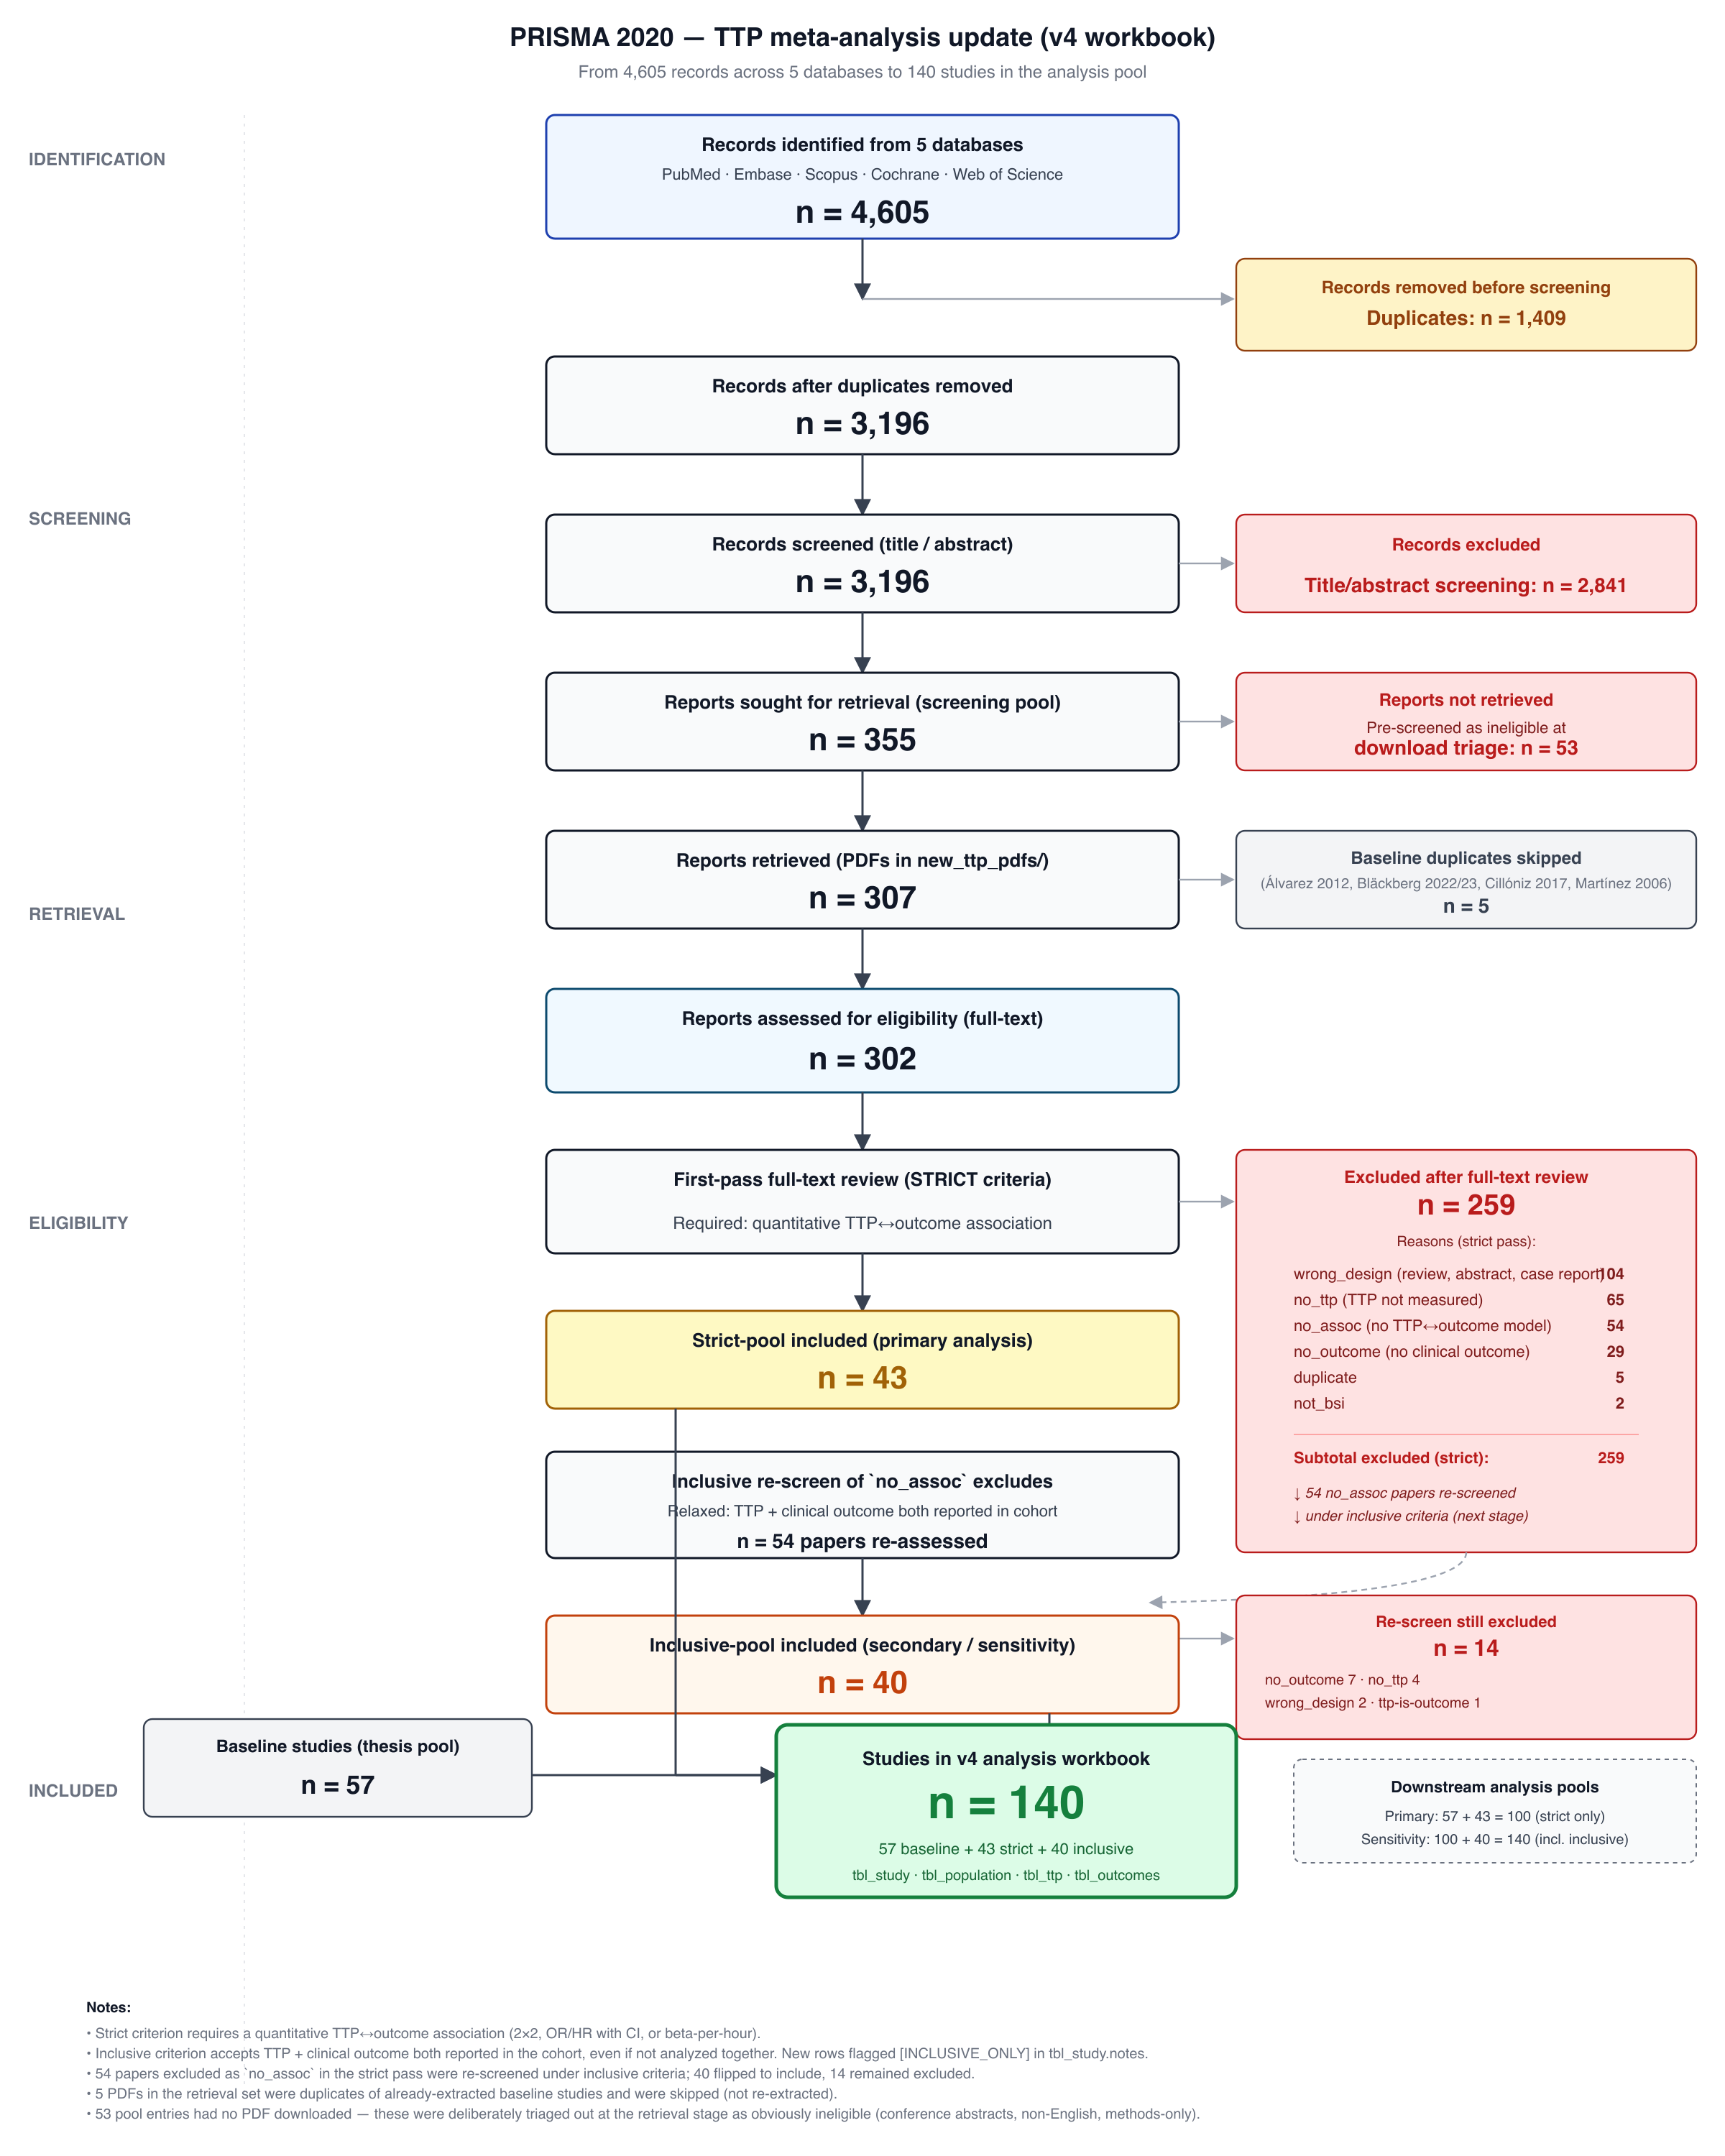
\includegraphics[width=1\linewidth,height=\textheight,keepaspectratio]{data/PRISMA_v4_update.png}

}

\caption{\label{fig-prisma}PRISMA 2020 flow diagram for the original
search and the May 2026 update.}

\end{figure}%

\subsection{Data extraction and risk of
bias}\label{data-extraction-and-risk-of-bias}

Data were extracted into a structured relational workbook with linked
tables for study characteristics, population, TTP reporting (continuous,
dichotomized, or categorical; units; cutpoints), and outcomes (events
and totals by TTP group, reported effect estimates, adjustment status,
and outcome definitions). TTP was recorded in hours. Where a study
reported both 2×2 data and an effect estimate, the 2×2 data were
preferred. The baseline 57 studies were extracted by the thesis author
{[}confirm whether extraction was independently verified{]}. For the
2026 update, full-text screening and data extraction were performed by a
large language model agent working from the full-text PDFs and the
written eligibility criteria and extraction codebook. Each of the 43
strict-pool extractions was then independently verified field by field
against the source PDF by a separate agent that had not performed the
original extraction; this led to 7 corrections before analysis. Studies
using TTP only as part of a catheter-related bloodstream infection case
definition were excluded from effect-size pooling. The human
contribution to screening and extraction decisions (spot-checking,
adjudication, or second human review) is described in the AI-use
statement below {[}confirm{]}, and we did not perform dual independent
human screening or report inter-rater agreement.

Risk of bias was assessed for every included study with the Quality in
Prognosis Studies (QUIPS) tool across six domains (participation,
attrition, prognostic factor measurement, outcome measurement,
confounding, and statistical analysis and reporting), each rated as low,
moderate, or high, with an overall rating per study
(\href{notebooks/rob.qmd}{notebook}). For the update these ratings were
generated by the extraction agent and were not independently re-rated by
a second human.

\subsection{Statistical analysis}\label{statistical-analysis}

Log odds ratios for mortality (short versus long TTP) were computed with
\texttt{metafor::escalc()} from 2×2 tables where available, otherwise
back-calculated from reported OR, HR, or RR with 95\% confidence
intervals. Effect sizes were pooled with a Bayesian random-effects model
(\texttt{brms}; study-level random intercepts) with weakly informative
priors (\(\mu \sim \mathcal{N}(0,1)\),
\(\tau \sim \text{Half-Cauchy}(0, 0.5)\)). Four chains of 4,000
iterations (1,000 warm-up) were run with \texttt{adapt\_delta\ =\ 0.99}.
Convergence was assessed with \(\hat{R}\) and effective sample sizes.
Secondary analyses examined pathogen class, TTP cutpoint
(meta-regression), publication bias, and a sensitivity pool that added
studies meeting a more inclusive criterion. All code and data are
available in the project repository.

\section{Results}\label{results}

\subsection{Study selection and
characteristics}\label{study-selection-and-characteristics}

The primary (strict) pool comprised 100 studies, of which 58 reported
mortality and contributed 72 mortality effect sizes. Overall risk of
bias (QUIPS) was low in 24, moderate in 62, high in 13, and critical in
1 studies (\href{notebooks/rob.qmd}{notebook}).

\subsection{Primary analysis}\label{primary-analysis}

Short TTP was associated with higher mortality (pooled OR 2.06 (95\%
CrI, 1.67 to 2.55); Figure~\ref{fig-forest}, Table~\ref{tbl-overall}).
The posterior probability that short TTP increases mortality was
100.0\%, and heterogeneity was substantial (median \(I^2\) = 62\%).

{

\begin{longtable}[]{@{}ll@{}}

\caption{\label{tbl-overall}Pooled effect of short vs long TTP on
mortality (OR \textgreater{} 1 = short TTP harmful). Primary pool only
(strict criterion).}

\tabularnewline

\toprule\noalign{}
Parameter & Value \\
\midrule\noalign{}
\endhead
\bottomrule\noalign{}
\endlastfoot
Median OR (short vs long TTP) & 2.06 \\
95\% credible interval & {[}1.67, 2.55{]} \\
95\% prediction interval (new study) & {[}0.50, 8.41{]} \\
P(short TTP harmful) & 100.0\% \\
Between-study SD (τ) & 0.69 \\
Heterogeneity (I²) & 62\% \\

\end{longtable}

}

\textsubscript{Source:
\href{https://lewis-id-lab.github.io/ttp-bacteremia-meta-analysis/notebooks/mortality-analysis-preview.html\#cell-tbl-overall}{Time-to-Positivity
and Mortality in Bacteremia}}

\begin{figure}[H]

\centering{

\pandocbounded{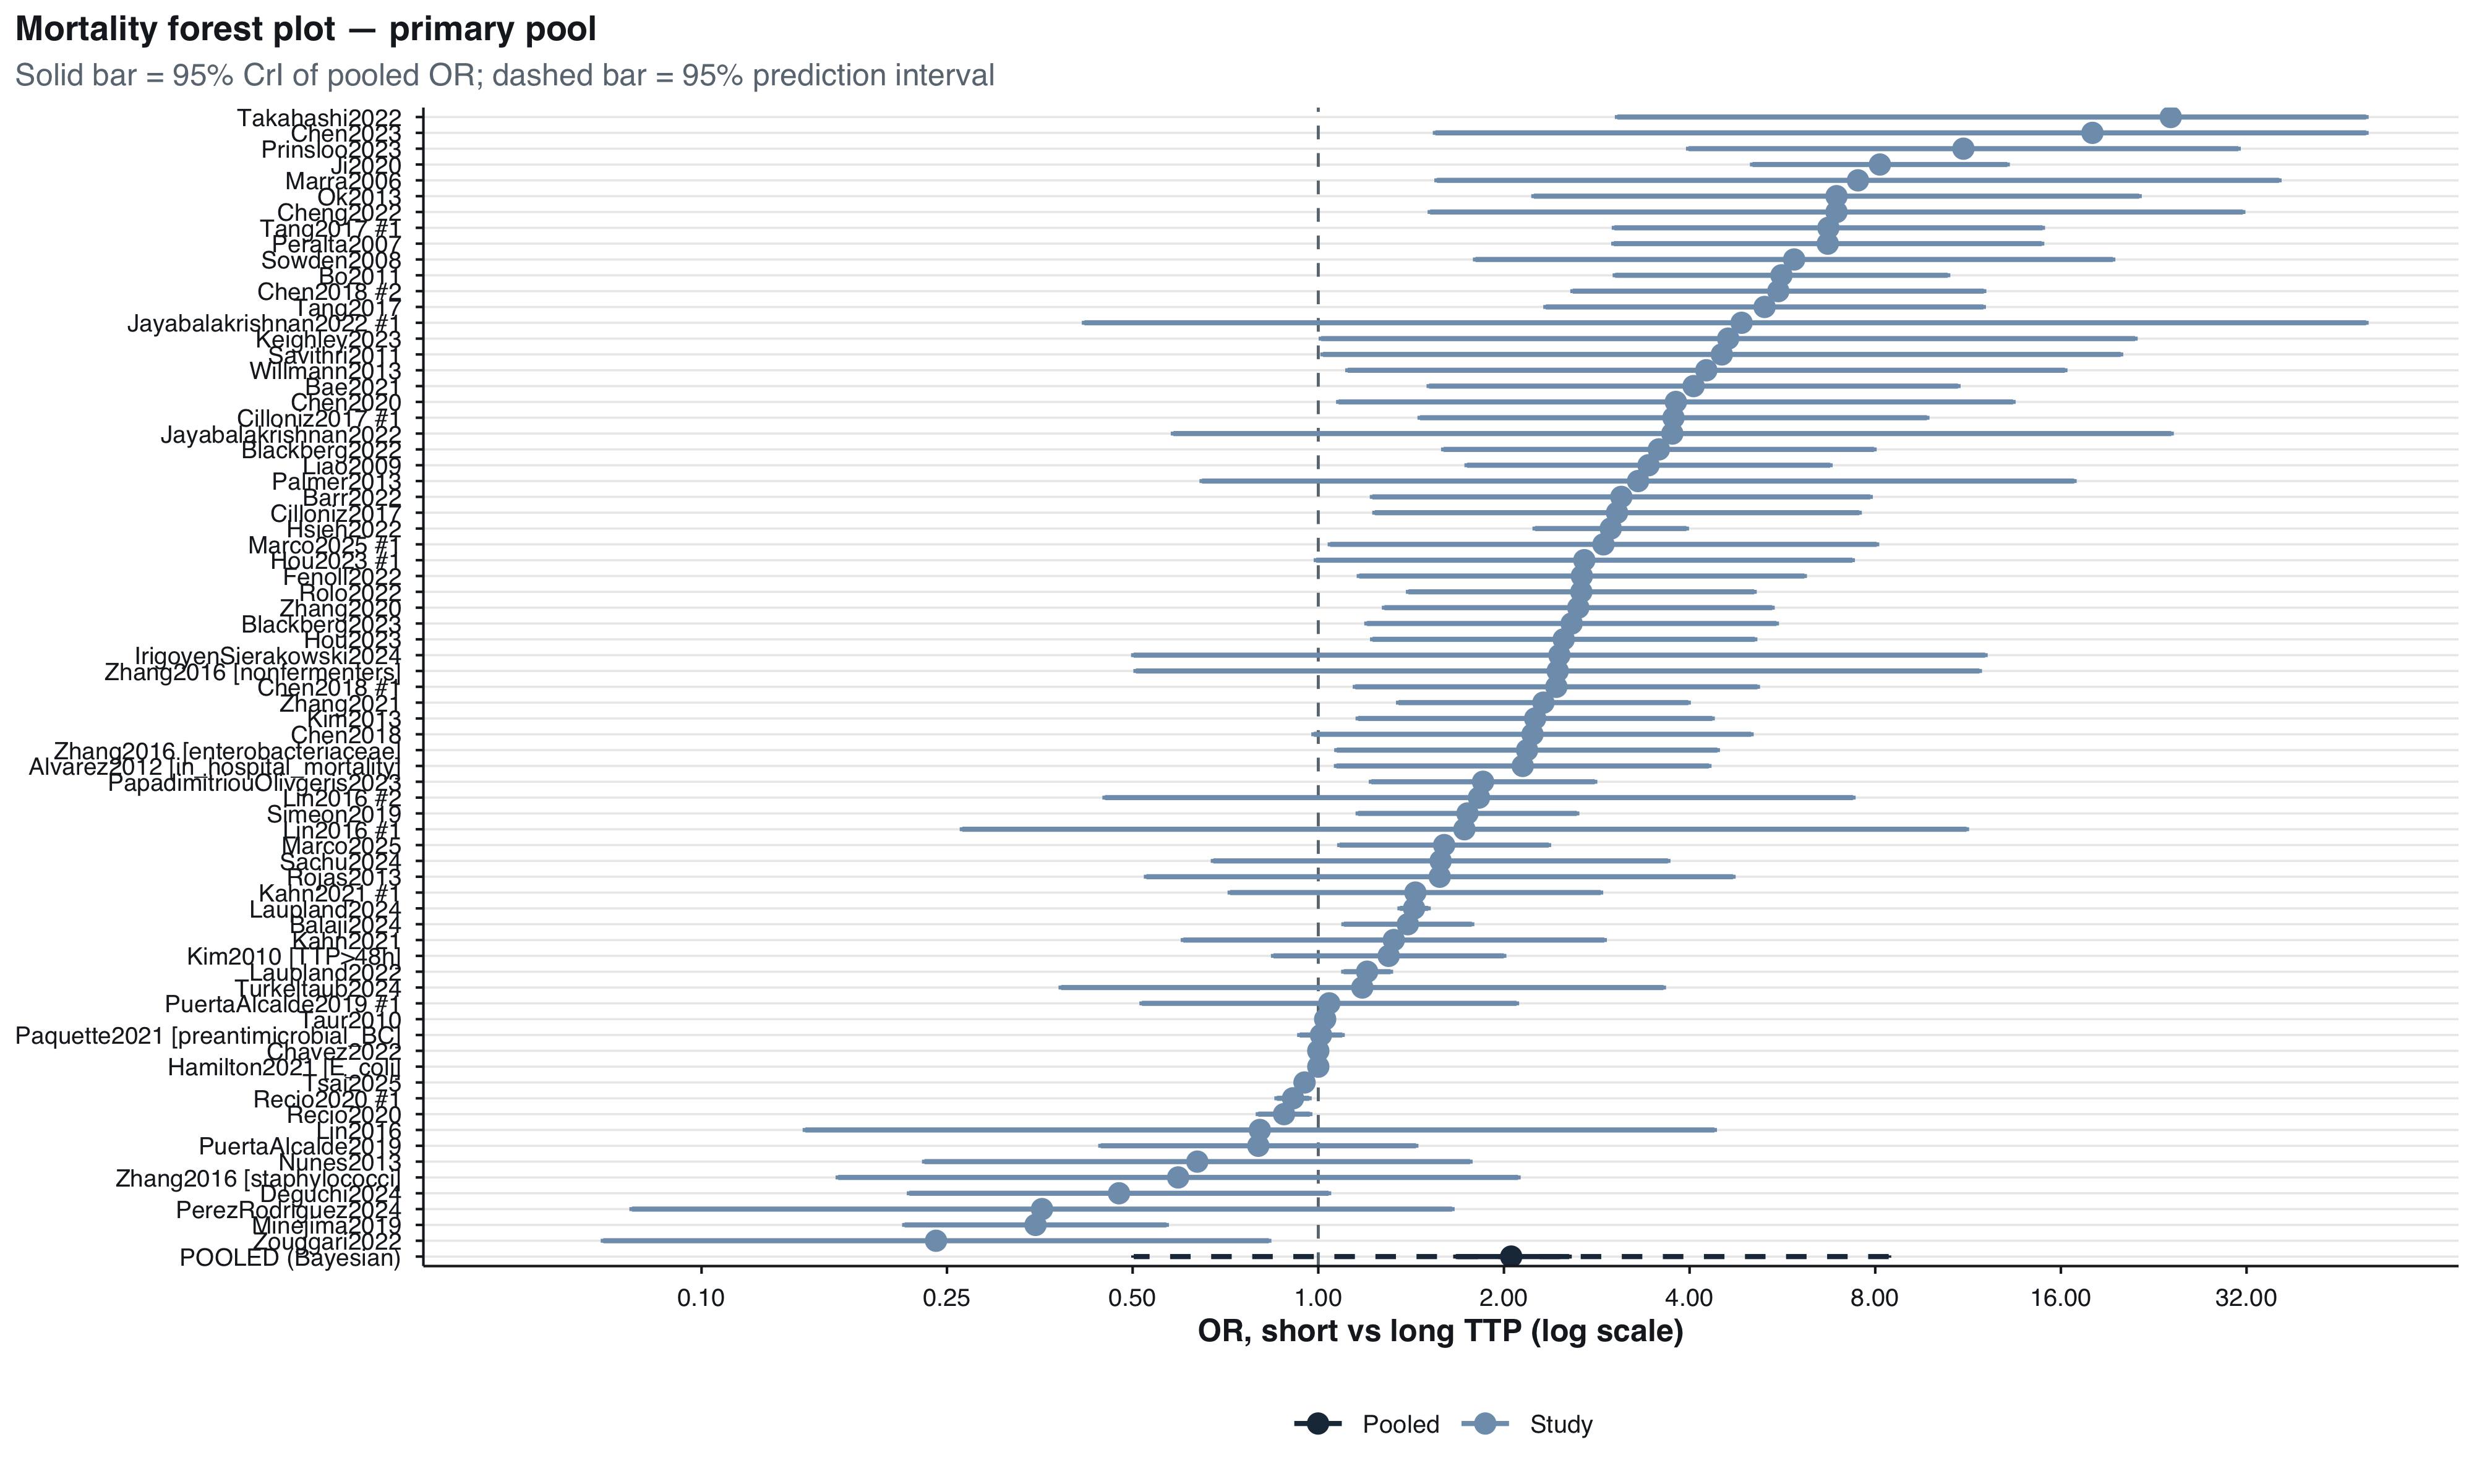
\includegraphics[keepaspectratio]{index_files/figure-latex/notebooks-mortality-analysis-fig-forest-output-2.png}}

}

\caption{\label{fig-forest}Forest plot of OR (short vs long TTP) on
mortality --- primary pool. Each row is a single effect size; multi-arm
studies appear multiple times. Pooled estimate from the Bayesian model
in dark navy.}

\end{figure}%

\textsubscript{Source:
\href{https://lewis-id-lab.github.io/ttp-bacteremia-meta-analysis/notebooks/mortality-analysis-preview.html\#cell-fig-forest}{Time-to-Positivity
and Mortality in Bacteremia}}

\subsection{Pathogen class}\label{pathogen-class}

\begin{figure}[H]

\centering{

\pandocbounded{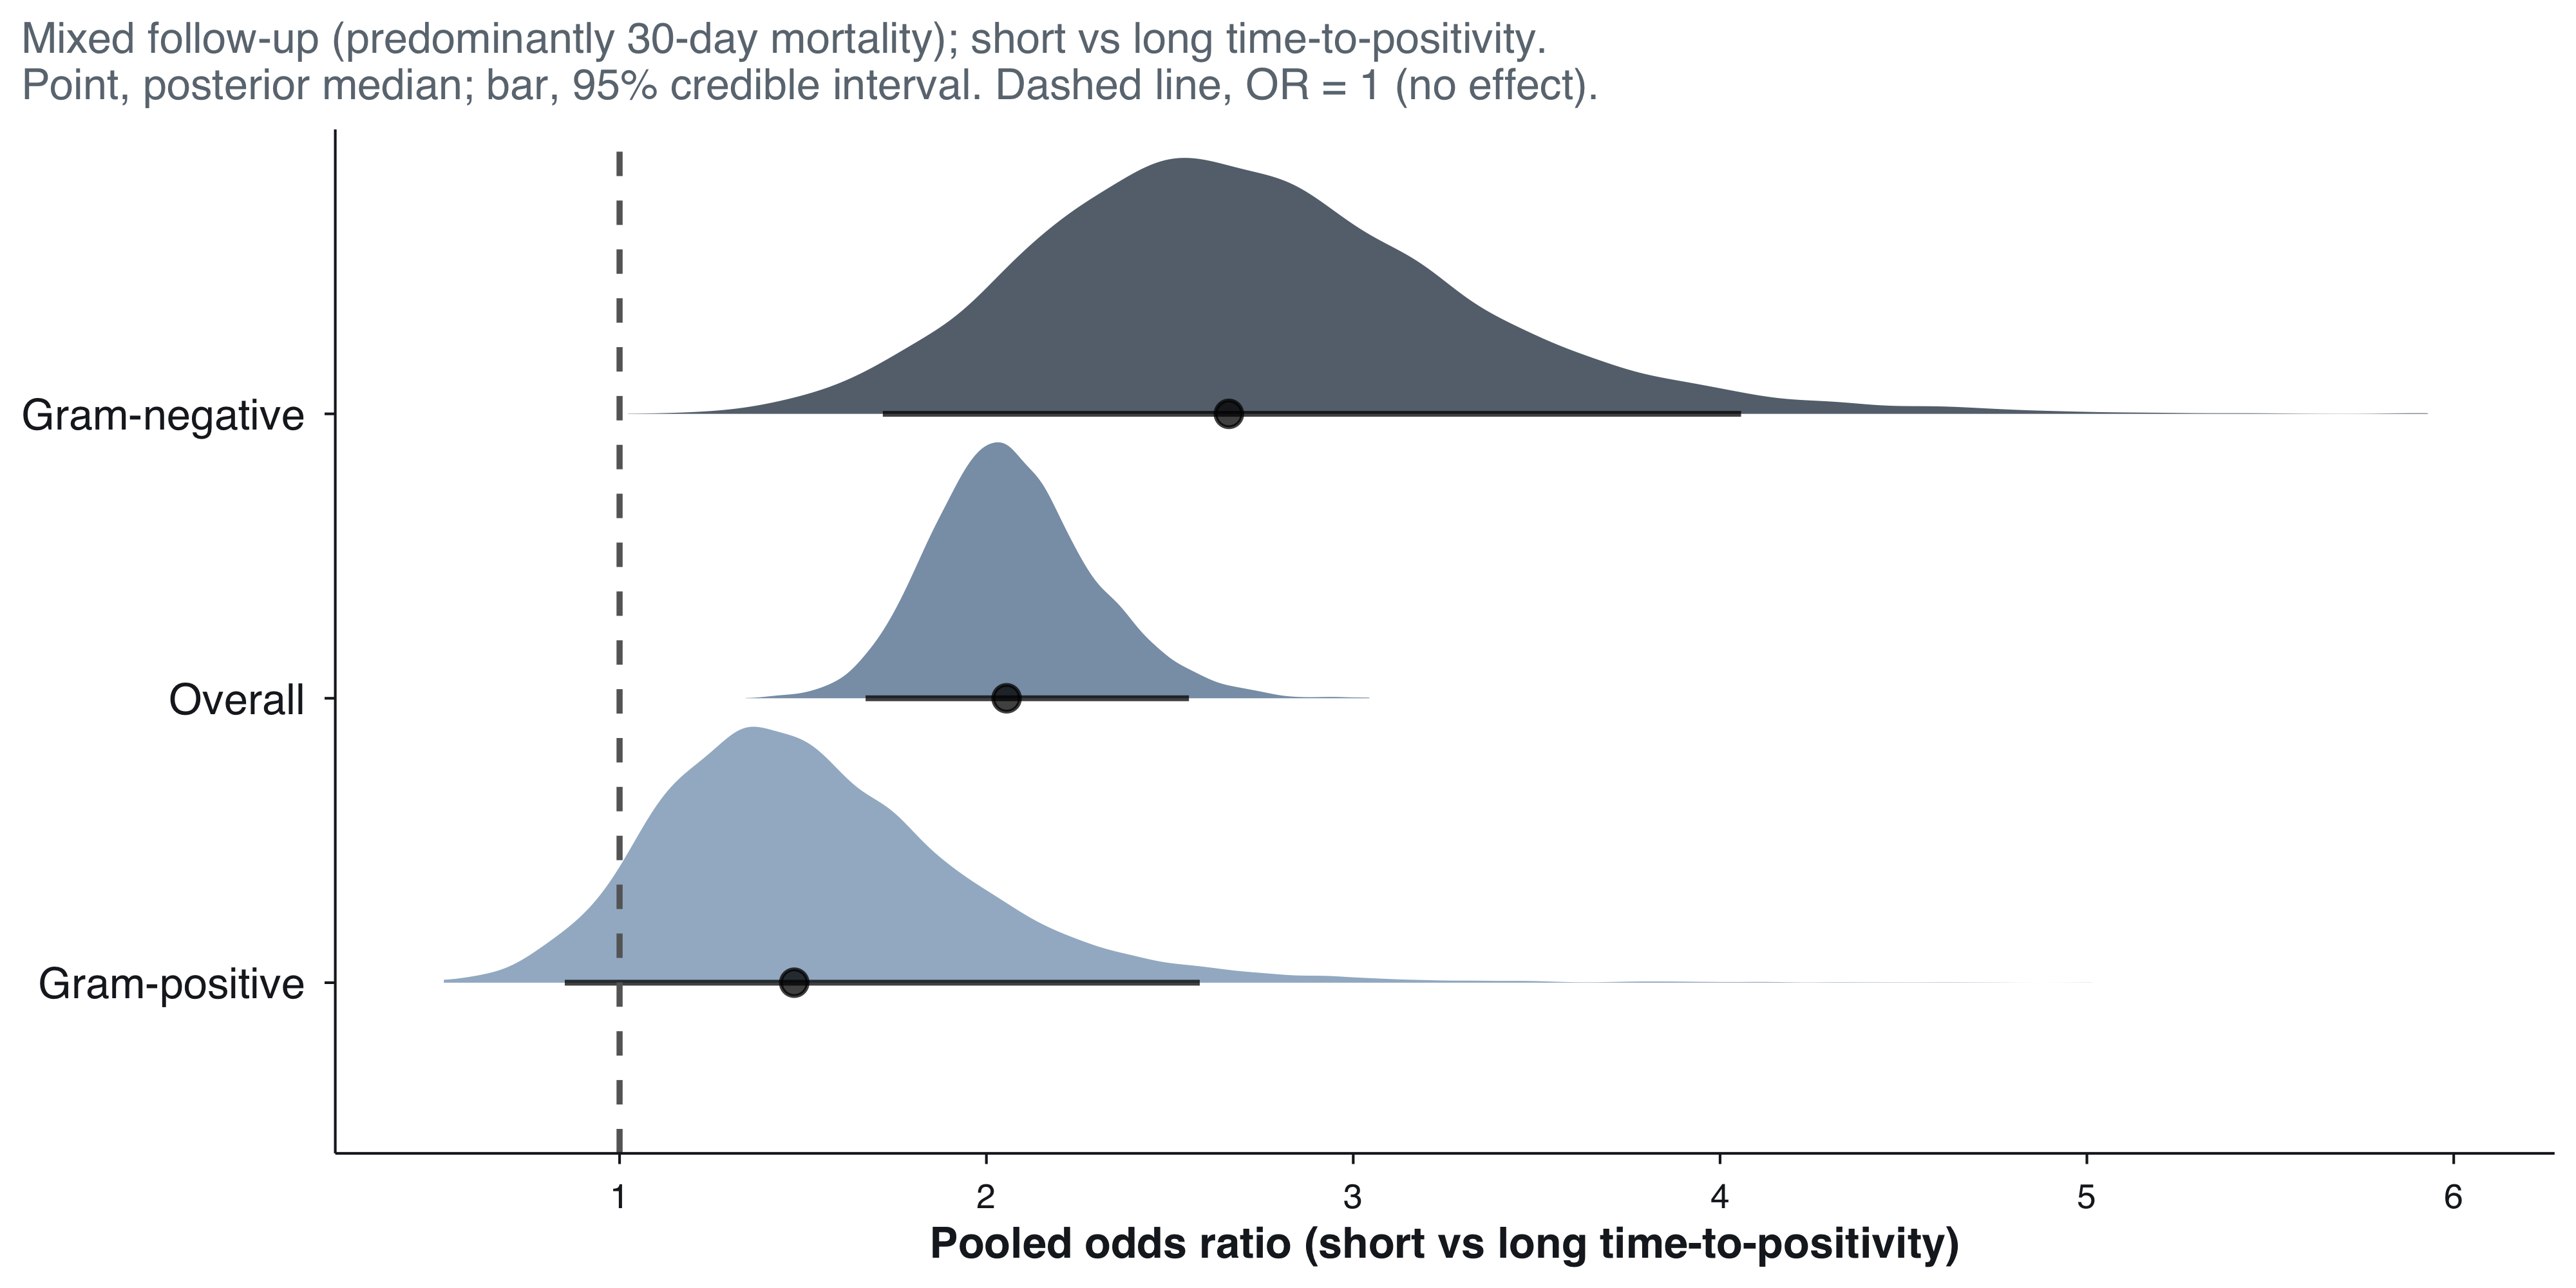
\includegraphics[keepaspectratio]{index_files/figure-latex/notebooks-mortality-analysis-fig-pathogen-posteriors-output-2.png}}

}

\caption{\label{fig-pathogen-posteriors}\textbf{Figure 1.} Posterior
distributions of the pooled odds ratio (OR) for all-cause mortality
comparing short versus long time-to-positivity (TTP), stratified by
pathogen class. Each density represents the full posterior from a
Bayesian random-effects meta-analysis (72 mortality effect sizes; 100
studies). The filled point marks the posterior median; the horizontal
bar spans the 95\% credible interval (CrI). The vertical dashed line
indicates OR = 1 (no effect). `Short' and `long' TTP were defined by
individual studies using study-specific thresholds (median cutpoint 12
h; range 2--72 h). Outcome was predominantly 30-day mortality. Overall:
OR = 2.06 (95\% CrI 1.67--2.55); Gram-negative: OR = 2.66 (95\% CrI
1.72--4.06); Gram-positive: OR = 1.48 (95\% CrI 0.85--2.58). OR
\textgreater{} 1 indicates higher mortality with shorter TTP.}

\end{figure}%

\textsubscript{Source:
\href{https://lewis-id-lab.github.io/ttp-bacteremia-meta-analysis/notebooks/mortality-analysis-preview.html\#cell-fig-pathogen-posteriors}{Time-to-Positivity
and Mortality in Bacteremia}}

Pathogen class was available for 52 of 72 mortality effect sizes
(Gram-negative, 26 effect sizes from 17 studies; Gram-positive, 13 from
11; fungal, 6 from 6; mixed or polymicrobial, 7 from 5). The remaining
20 effect sizes had no pathogen classification and were excluded from
the stratified models. Short TTP was associated with higher mortality in
Gram-negative bacteremia (OR 2.66 (95\% CrI, 1.72 to 4.06)) and, with a
smaller point estimate and a credible interval that included 1, in
Gram-positive bacteremia (OR 1.48 (95\% CrI, 0.85 to 2.58);
Figure~\ref{fig-pathogen-posteriors}, Table~\ref{tbl-subgroup}). In a
meta-regression with both classes, the odds ratio in Gram-positive
studies was 0.61 times that in Gram-negative studies (95\% CrI 0.36 to
1.02), with a posterior probability of 97\% that the association is
weaker in Gram-positive studies. This interval is wide and just includes
1, so the evidence for a difference between classes is suggestive rather
than conclusive. For fungal bacteremia the pooled estimate was imprecise
(OR 1.31 (95\% CrI, 0.92 to 2.12), 6 studies). Heterogeneity remained
considerable within both Gram-negative (median \(I^2\) 61\%) and
Gram-positive (74\%) strata.

{

\begin{longtable}[]{@{}lllll@{}}

\caption{\label{tbl-subgroup}Pooled OR by pathogen subgroup.}

\tabularnewline

\toprule\noalign{}
Subgroup & N effect sizes & Median OR & 95\% CrI & P(short TTP
harmful) \\
\midrule\noalign{}
\endhead
\bottomrule\noalign{}
\endlastfoot
Gram-positive & 13 & 1.48 & {[}0.85, 2.58{]} & 92.7\% \\
Gram-negative & 26 & 2.66 & {[}1.72, 4.06{]} & 100.0\% \\

\end{longtable}

}

\textsubscript{Source:
\href{https://lewis-id-lab.github.io/ttp-bacteremia-meta-analysis/notebooks/mortality-analysis-preview.html\#cell-tbl-subgroup}{Time-to-Positivity
and Mortality in Bacteremia}}

\subsection{TTP cutpoint}\label{ttp-cutpoint}

A TTP cutpoint was reported for 42 of 72 mortality effect sizes (29
studies); the remainder had no cutpoint recorded in the extraction
database. Cutpoints ranged from 2 to 72 h (median 12 h). Across all
effect sizes with a cutpoint, the log odds ratio changed by -0.035 (95\%
CrI, -0.056 to -0.015) per additional hour, so higher thresholds were
associated with weaker associations (Figure~\ref{fig-cutpoint}). When
the analysis was restricted to cutpoints of 24 h or less, the slope was
attenuated and its interval included zero (-0.024 (95\% CrI, -0.075 to
0.028)), so the gradient depends on the few studies using long
thresholds.

Within pathogen class the pattern differed. Among Gram-negative effect
sizes (median cutpoint 10 h) the slope was positive (0.062 (95\% CrI,
-0.005 to 0.130); Table~\ref{tbl-gneg-cutpoint}), whereas among
Gram-positive effect sizes it was negative with an interval that
included zero (-0.029 (95\% CrI, -0.058 to 0.004);
Table~\ref{tbl-gpos-cutpoint}). The overall negative gradient therefore
does not hold within Gram-negative bacteremia, and these class-specific
analyses rest on small numbers of effect sizes.

\begin{figure}[H]

\centering{

\pandocbounded{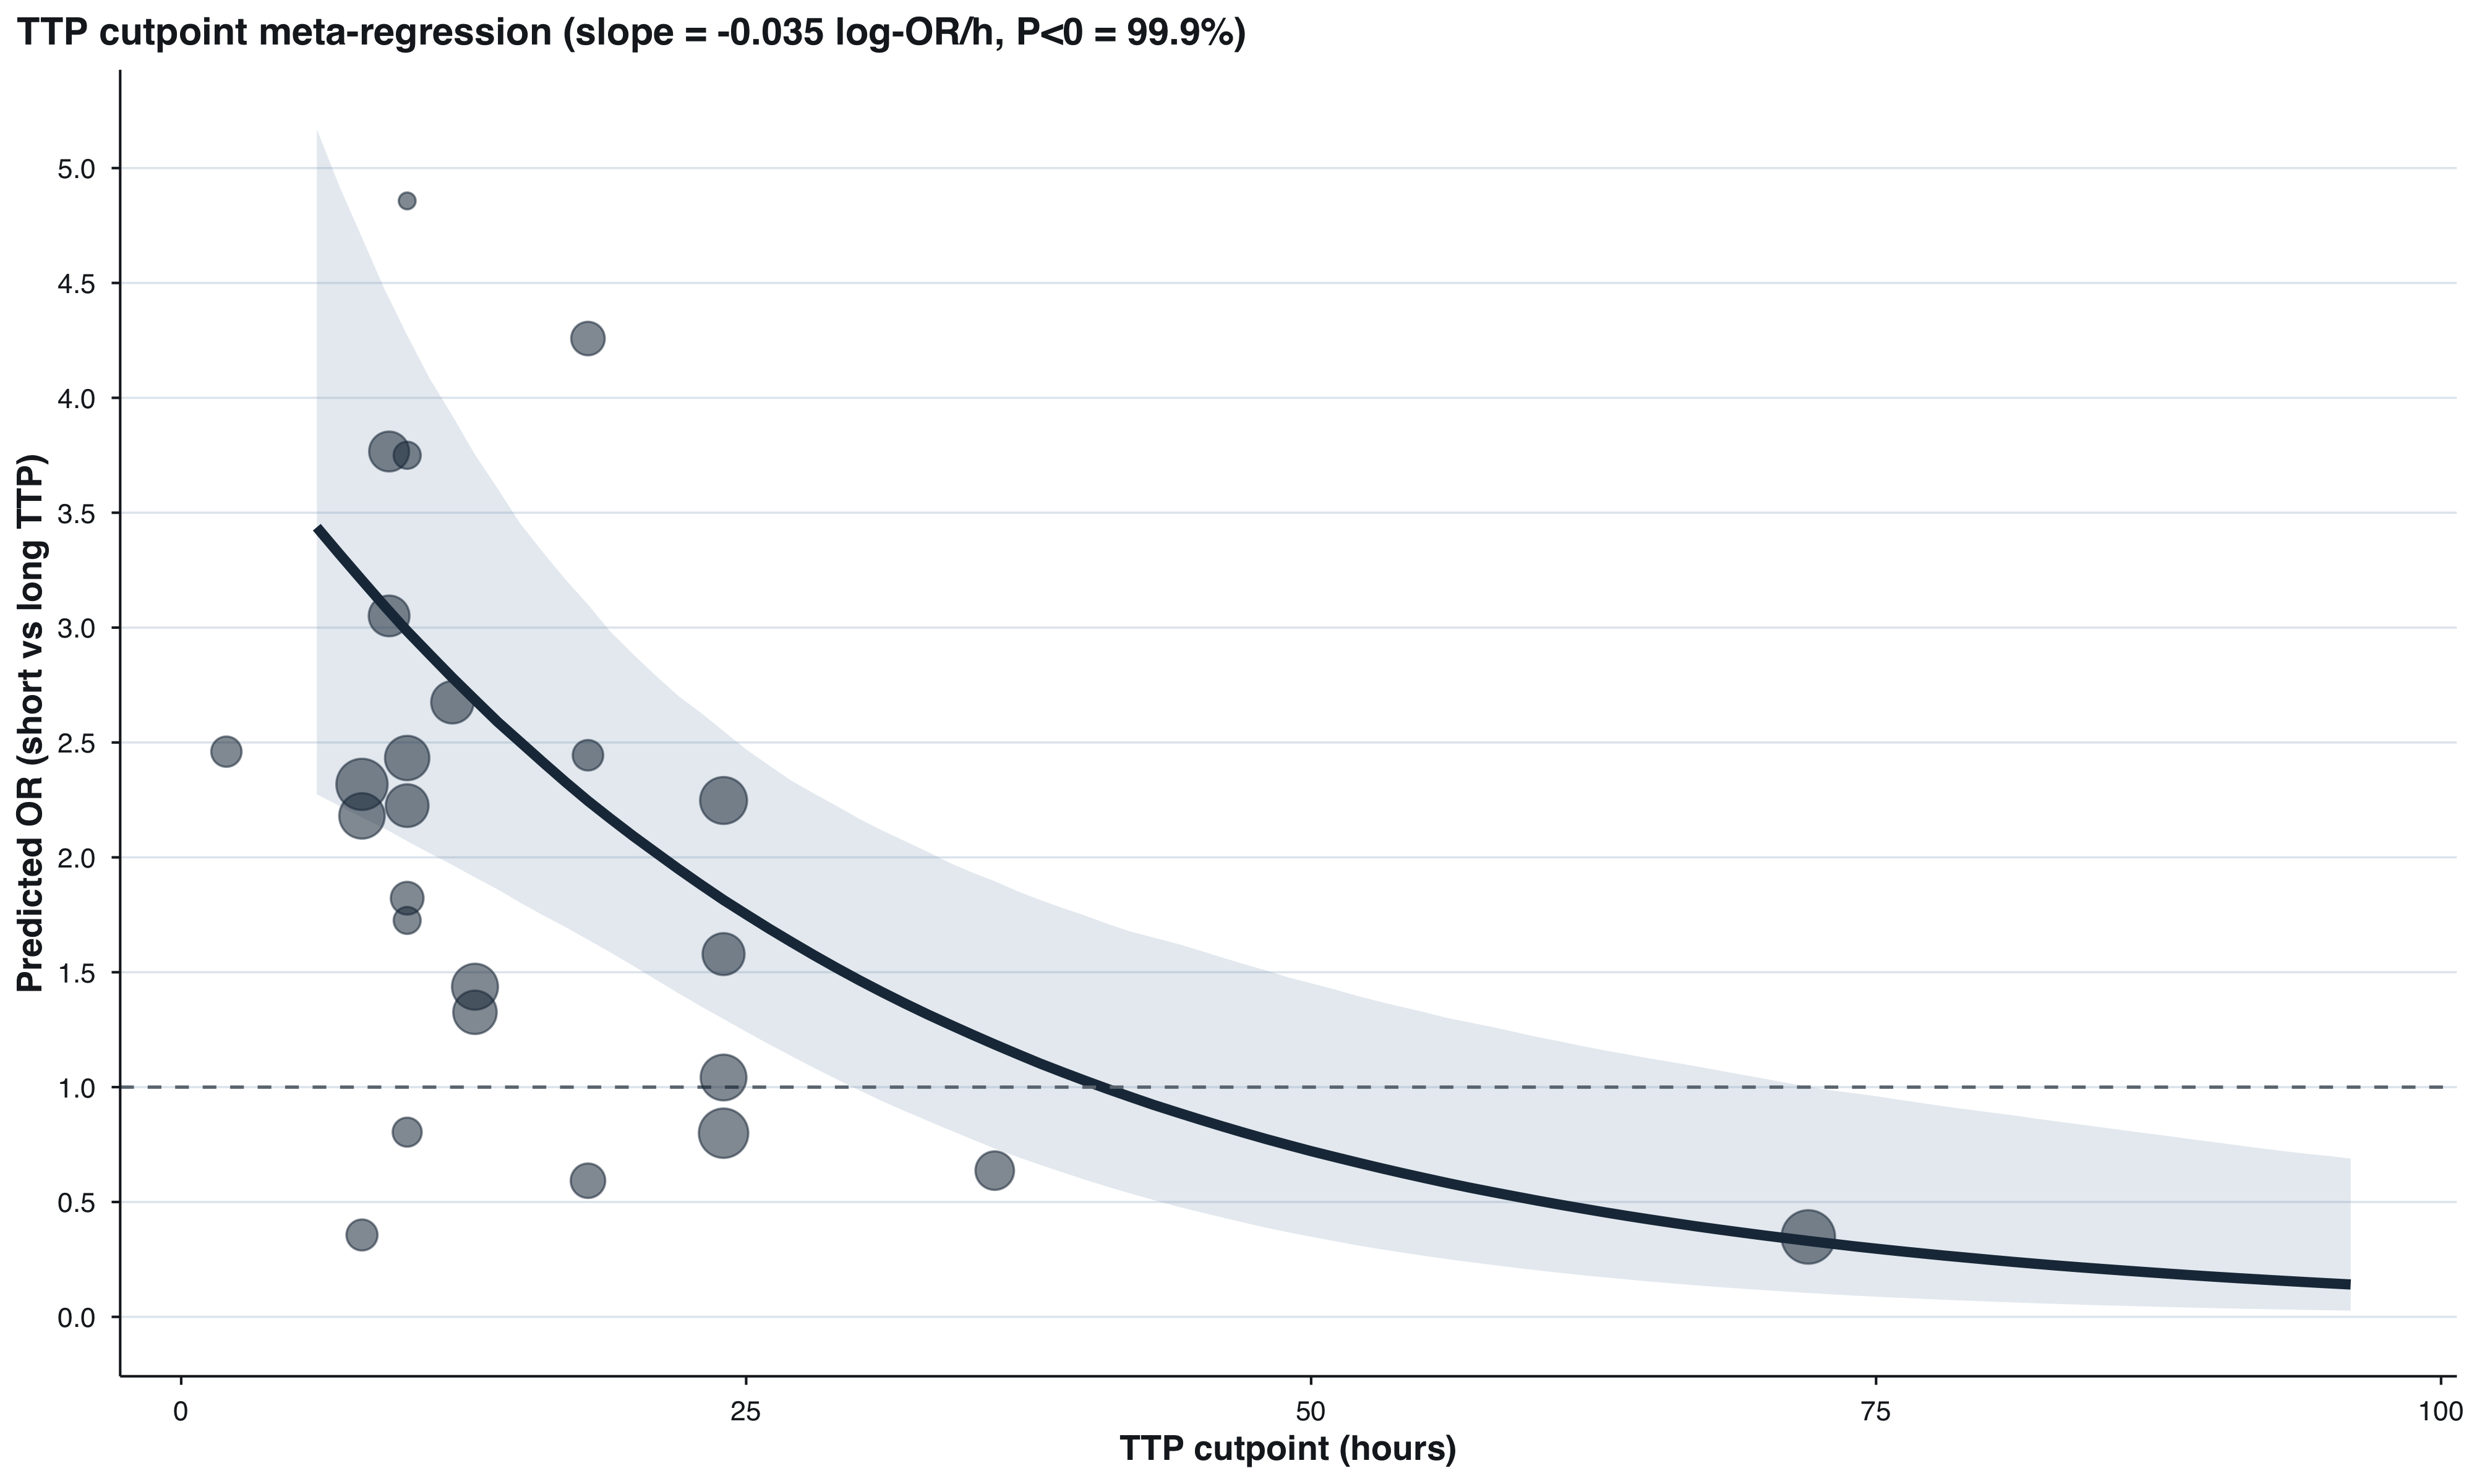
\includegraphics[keepaspectratio]{index_files/figure-latex/notebooks-mortality-analysis-fig-cutpoint-output-2.png}}

}

\caption{\label{fig-cutpoint}TTP cutpoint meta-regression. The line is
the Bayesian posterior median predicted OR by cutpoint; ribbon is the
95\% CrI. Dark points are observed 2×2-derived effect sizes (size ∝
precision).}

\end{figure}%

\textsubscript{Source:
\href{https://lewis-id-lab.github.io/ttp-bacteremia-meta-analysis/notebooks/mortality-analysis-preview.html\#cell-fig-cutpoint}{Time-to-Positivity
and Mortality in Bacteremia}}

{

\begin{longtable}[]{@{}llll@{}}

\caption{\label{tbl-gneg-cutpoint}Gram-negative cutpoint meta-regression
slope and predicted OR at key thresholds.}

\tabularnewline

\toprule\noalign{}
Parameter & Estimate & 95\% CrI & P(direction) \\
\midrule\noalign{}
\endhead
\bottomrule\noalign{}
\endlastfoot
Slope (log-OR per hour above median) & 0.062 & {[}-0.005, 0.130{]} &
96.8\% \\
Predicted OR at cutpoint 8 h & 3.03 & {[}2.02, 4.52{]} & 100.0\% \\
Predicted OR at cutpoint 10 h & 3.43 & {[}2.40, 4.87{]} & 100.0\% \\
Predicted OR at cutpoint 13 h & 4.14 & {[}2.84, 5.93{]} & 100.0\% \\
Predicted OR at cutpoint 18 h & 5.65 & {[}3.17, 9.95{]} & 100.0\% \\

\end{longtable}

}

\textsubscript{Source:
\href{https://lewis-id-lab.github.io/ttp-bacteremia-meta-analysis/notebooks/mortality-analysis-preview.html\#cell-tbl-gneg-cutpoint}{Time-to-Positivity
and Mortality in Bacteremia}}

{

\begin{longtable}[]{@{}llll@{}}

\caption{\label{tbl-gpos-cutpoint}Gram-positive cutpoint
meta-regression: slope comparison between full model and sensitivity
analysis excluding Minejima2019 (72 h).}

\tabularnewline

\toprule\noalign{}
Model & N studies & Slope (log-OR/h) & P(slope \textless{} 0) \\
\midrule\noalign{}
\endhead
\bottomrule\noalign{}
\endlastfoot
Full (8--72 h) & 7 & -0.029 {[}-0.058, 0.004{]} & 96.5\% \\
Sensitivity (excl. Minejima2019) & 6 & -0.081 {[}-0.323, 0.214{]} &
75.4\% \\

\end{longtable}

}

\textsubscript{Source:
\href{https://lewis-id-lab.github.io/ttp-bacteremia-meta-analysis/notebooks/mortality-analysis-preview.html\#cell-tbl-gpos-cutpoint}{Time-to-Positivity
and Mortality in Bacteremia}}

\subsection{Publication bias}\label{publication-bias}

The funnel plot of mortality effect sizes was asymmetric
(Figure~\ref{fig-funnel}). Egger's regression test indicated small-study
effects (t = 6.19, df = 70, p \textless{} 0.0001;
Table~\ref{tbl-egger}), and the regression-based estimate for a study
with zero standard error was close to no association (OR 0.99; 95\% CI
0.97 to 1.01). Begg's rank correlation test did not detect asymmetry (p
= 0.47). The trim-and-fill method imputed 19 missing studies and gave an
adjusted pooled OR of 1.51 (95\% CI, 1.23 to 1.86), lower than the
unadjusted frequentist estimate (OR 2.05). These tests treat all effect
sizes as independent, assume that asymmetry is due to selective
reporting, and have limited reliability when heterogeneity is high, so
they cannot distinguish publication bias from genuine heterogeneity,
such as larger associations in smaller studies that used more extreme or
optimized cutpoints. The evidence nevertheless suggests that the pooled
association may be overestimated.

\begin{figure}[H]

\centering{

\pandocbounded{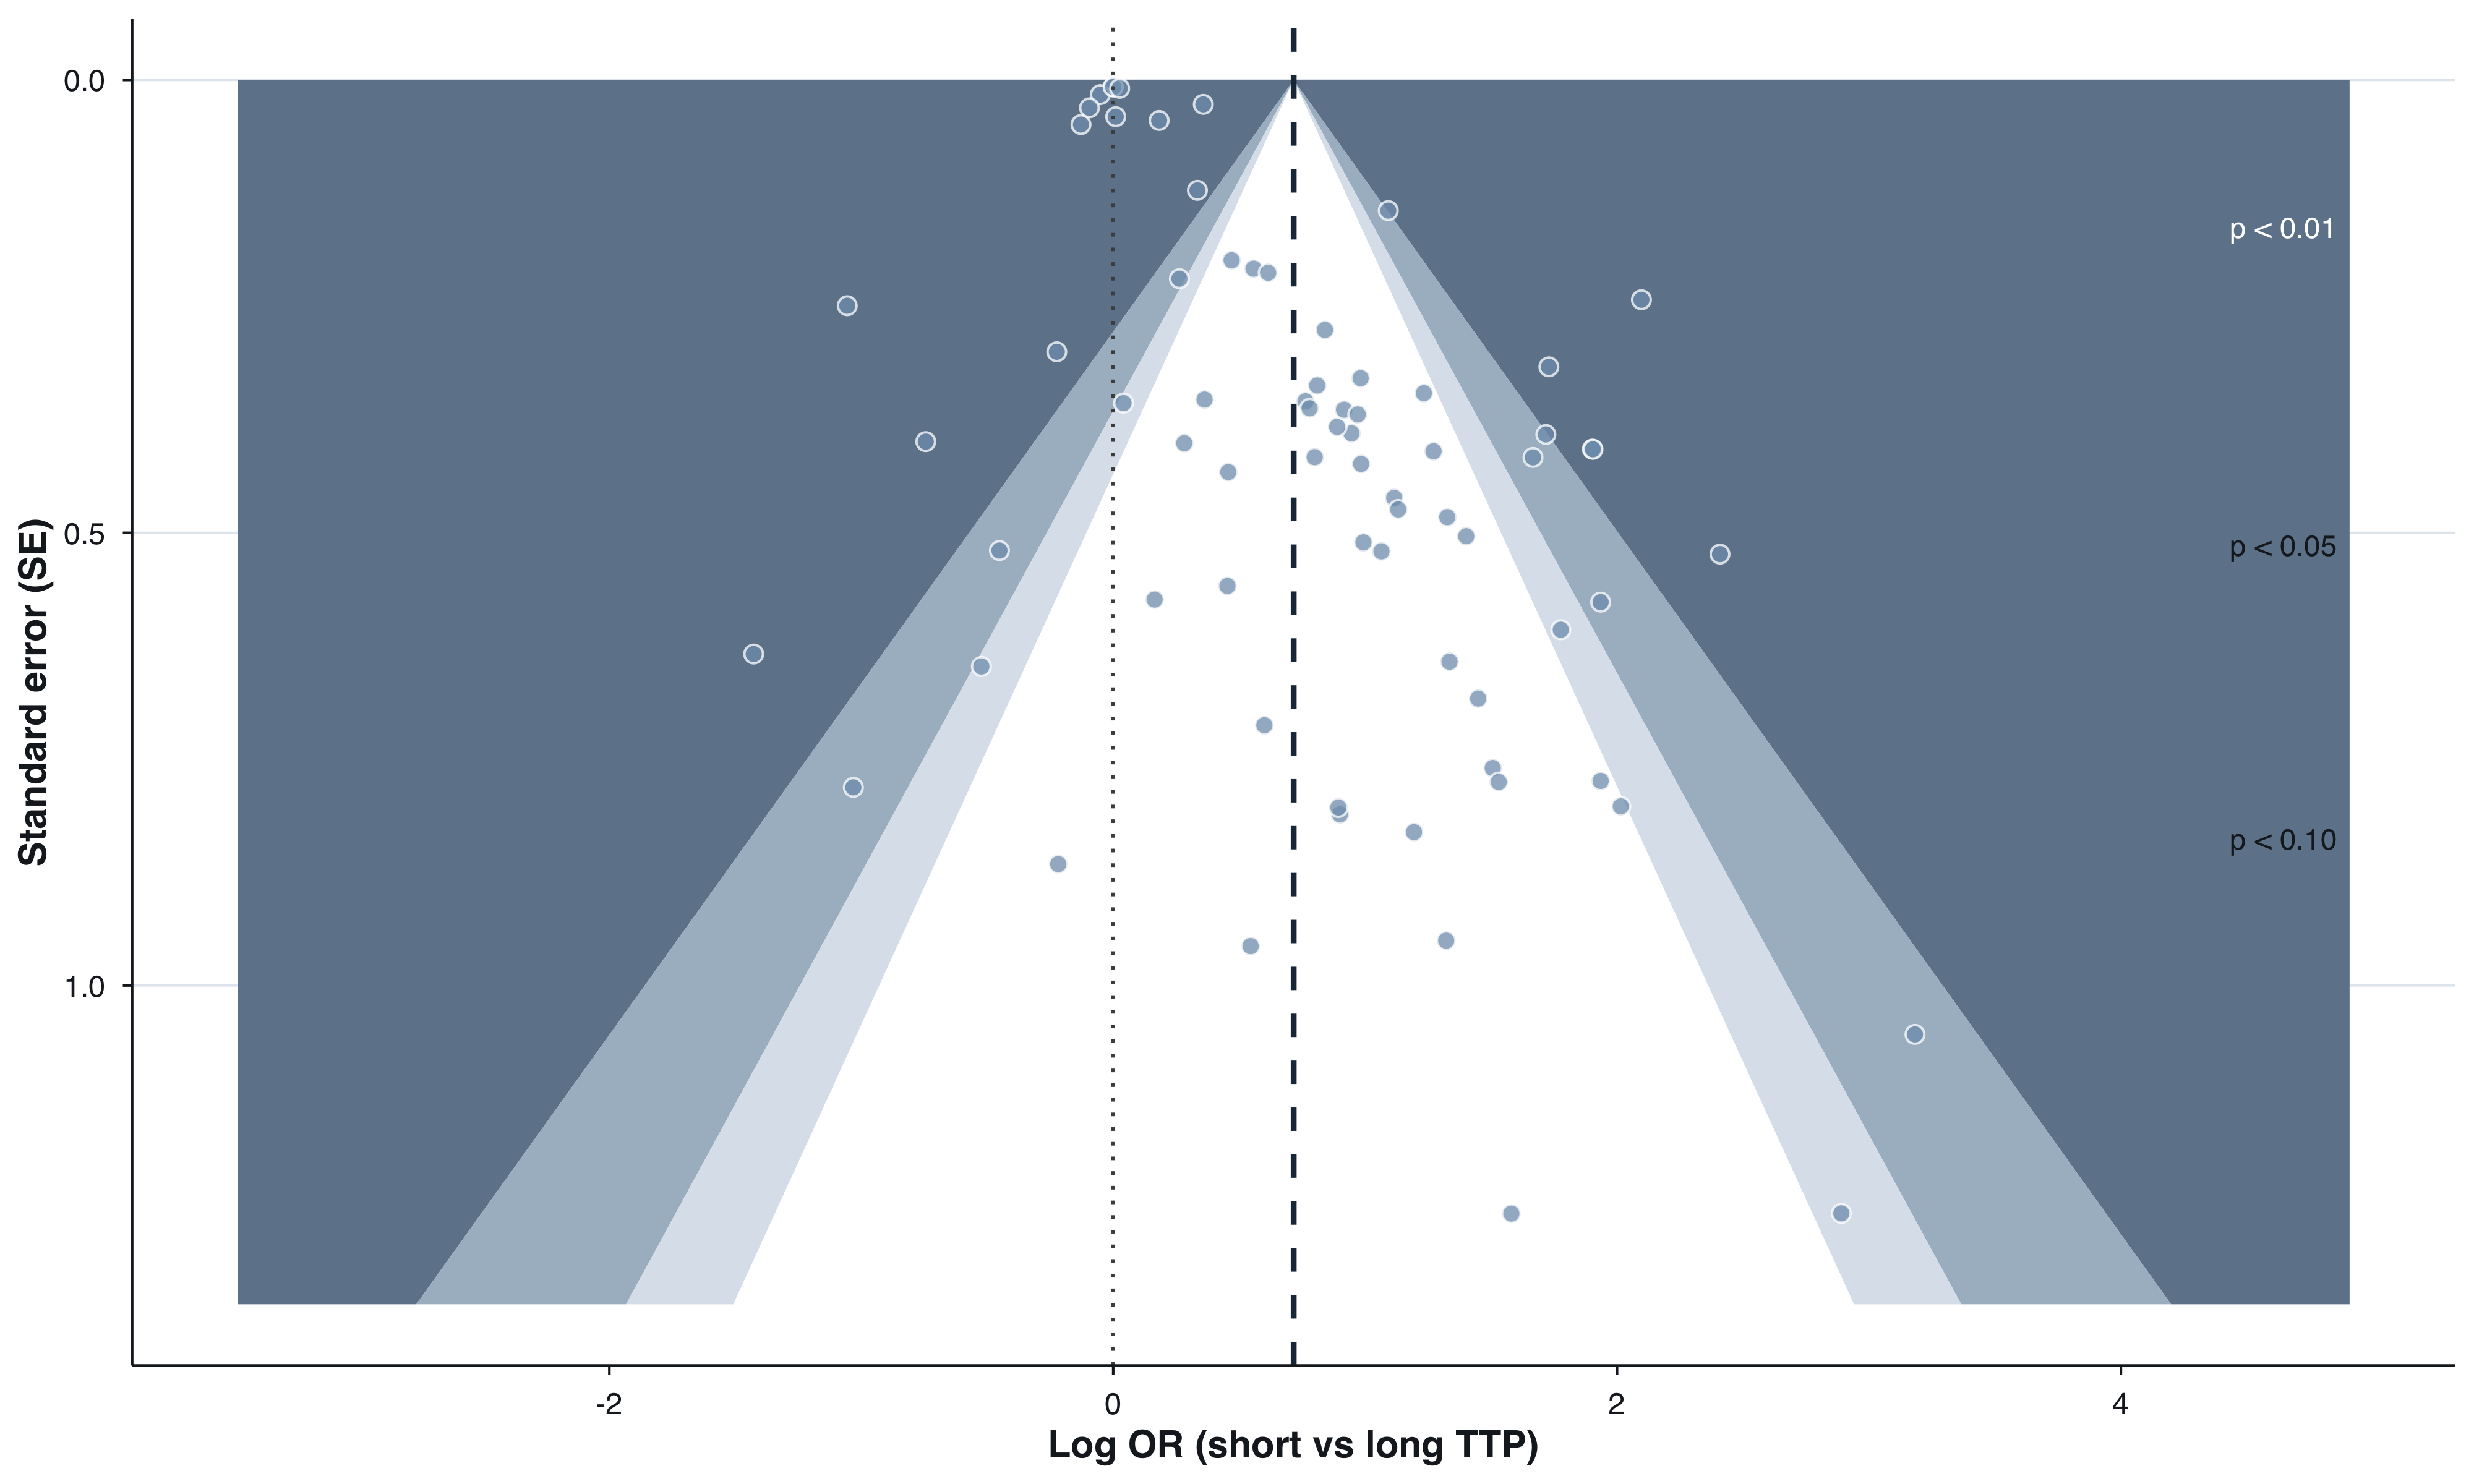
\includegraphics[keepaspectratio]{index_files/figure-latex/notebooks-mortality-analysis-fig-funnel-output-1.png}}

}

\caption{\label{fig-funnel}Contour-enhanced funnel plot (primary pool,
mortality). Studies in white zones are not statistically significant at
the labelled threshold; shaded outer zones indicate increasing levels of
significance. Asymmetry toward the right (short TTP harmful) would
suggest positive-result publication bias.}

\end{figure}%

\textsubscript{Source:
\href{https://lewis-id-lab.github.io/ttp-bacteremia-meta-analysis/notebooks/mortality-analysis-preview.html\#cell-fig-funnel}{Time-to-Positivity
and Mortality in Bacteremia}}

{

\begin{longtable}[]{@{}ll@{}}

\caption{\label{tbl-egger}Egger's regression test for funnel-plot
asymmetry (primary pool, mortality; metafor::regtest, weighted
regression on the standard error). The t-statistic tests asymmetry; the
limit estimate is the predicted effect for a hypothetical study with
zero standard error.}

\tabularnewline

\toprule\noalign{}
Statistic & Value \\
\midrule\noalign{}
\endhead
\bottomrule\noalign{}
\endlastfoot
Asymmetry test t-statistic & 6.19 \\
df & 70 \\
p-value & \textless1e-04 \\
Limit estimate as SE -\textgreater{} 0 (log OR) & -0.010 \\
95\% CI (log OR) & {[}-0.034, 0.014{]} \\
Limit estimate as SE -\textgreater{} 0 (OR) & 0.99 \\

\end{longtable}

}

\textsubscript{Source:
\href{https://lewis-id-lab.github.io/ttp-bacteremia-meta-analysis/notebooks/mortality-analysis-preview.html\#cell-tbl-egger}{Time-to-Positivity
and Mortality in Bacteremia}}

\subsection{Sensitivity analyses}\label{sensitivity-analyses}

Adding the studies that met only the inclusive criterion increased the
number of studies reporting mortality to 67 (84 effect sizes) and gave a
pooled OR of 1.92 (95\% CrI, 1.58 to 2.35), similar to the primary
estimate (Figure~\ref{fig-sens-inc}). Pooled estimates by data source
were consistent in direction. Relative to 2×2-derived effect sizes (49
effect sizes), the log odds ratio for effect sizes back-calculated from
adjusted reported estimates (15 effect sizes) was -0.26 (95\% CrI, -0.68
to 0.16) and for unadjusted reported estimates (8 effect sizes) was
-0.12 (95\% CrI, -0.62 to 0.38). Both intervals included zero. Directly
comparing unadjusted with adjusted reported estimates, the difference in
log odds ratio was 0.12 (95\% CrI, -0.39 to 0.62). Association strength
tended to decrease with publication year (change in log odds ratio per
year, -0.04 (95\% CrI, -0.08 to 0.00)), with an interval that only just
included zero. None of these moderator analyses showed a clear
difference, but all were underpowered relative to the observed
heterogeneity.

\begin{figure}[H]

\centering{

\pandocbounded{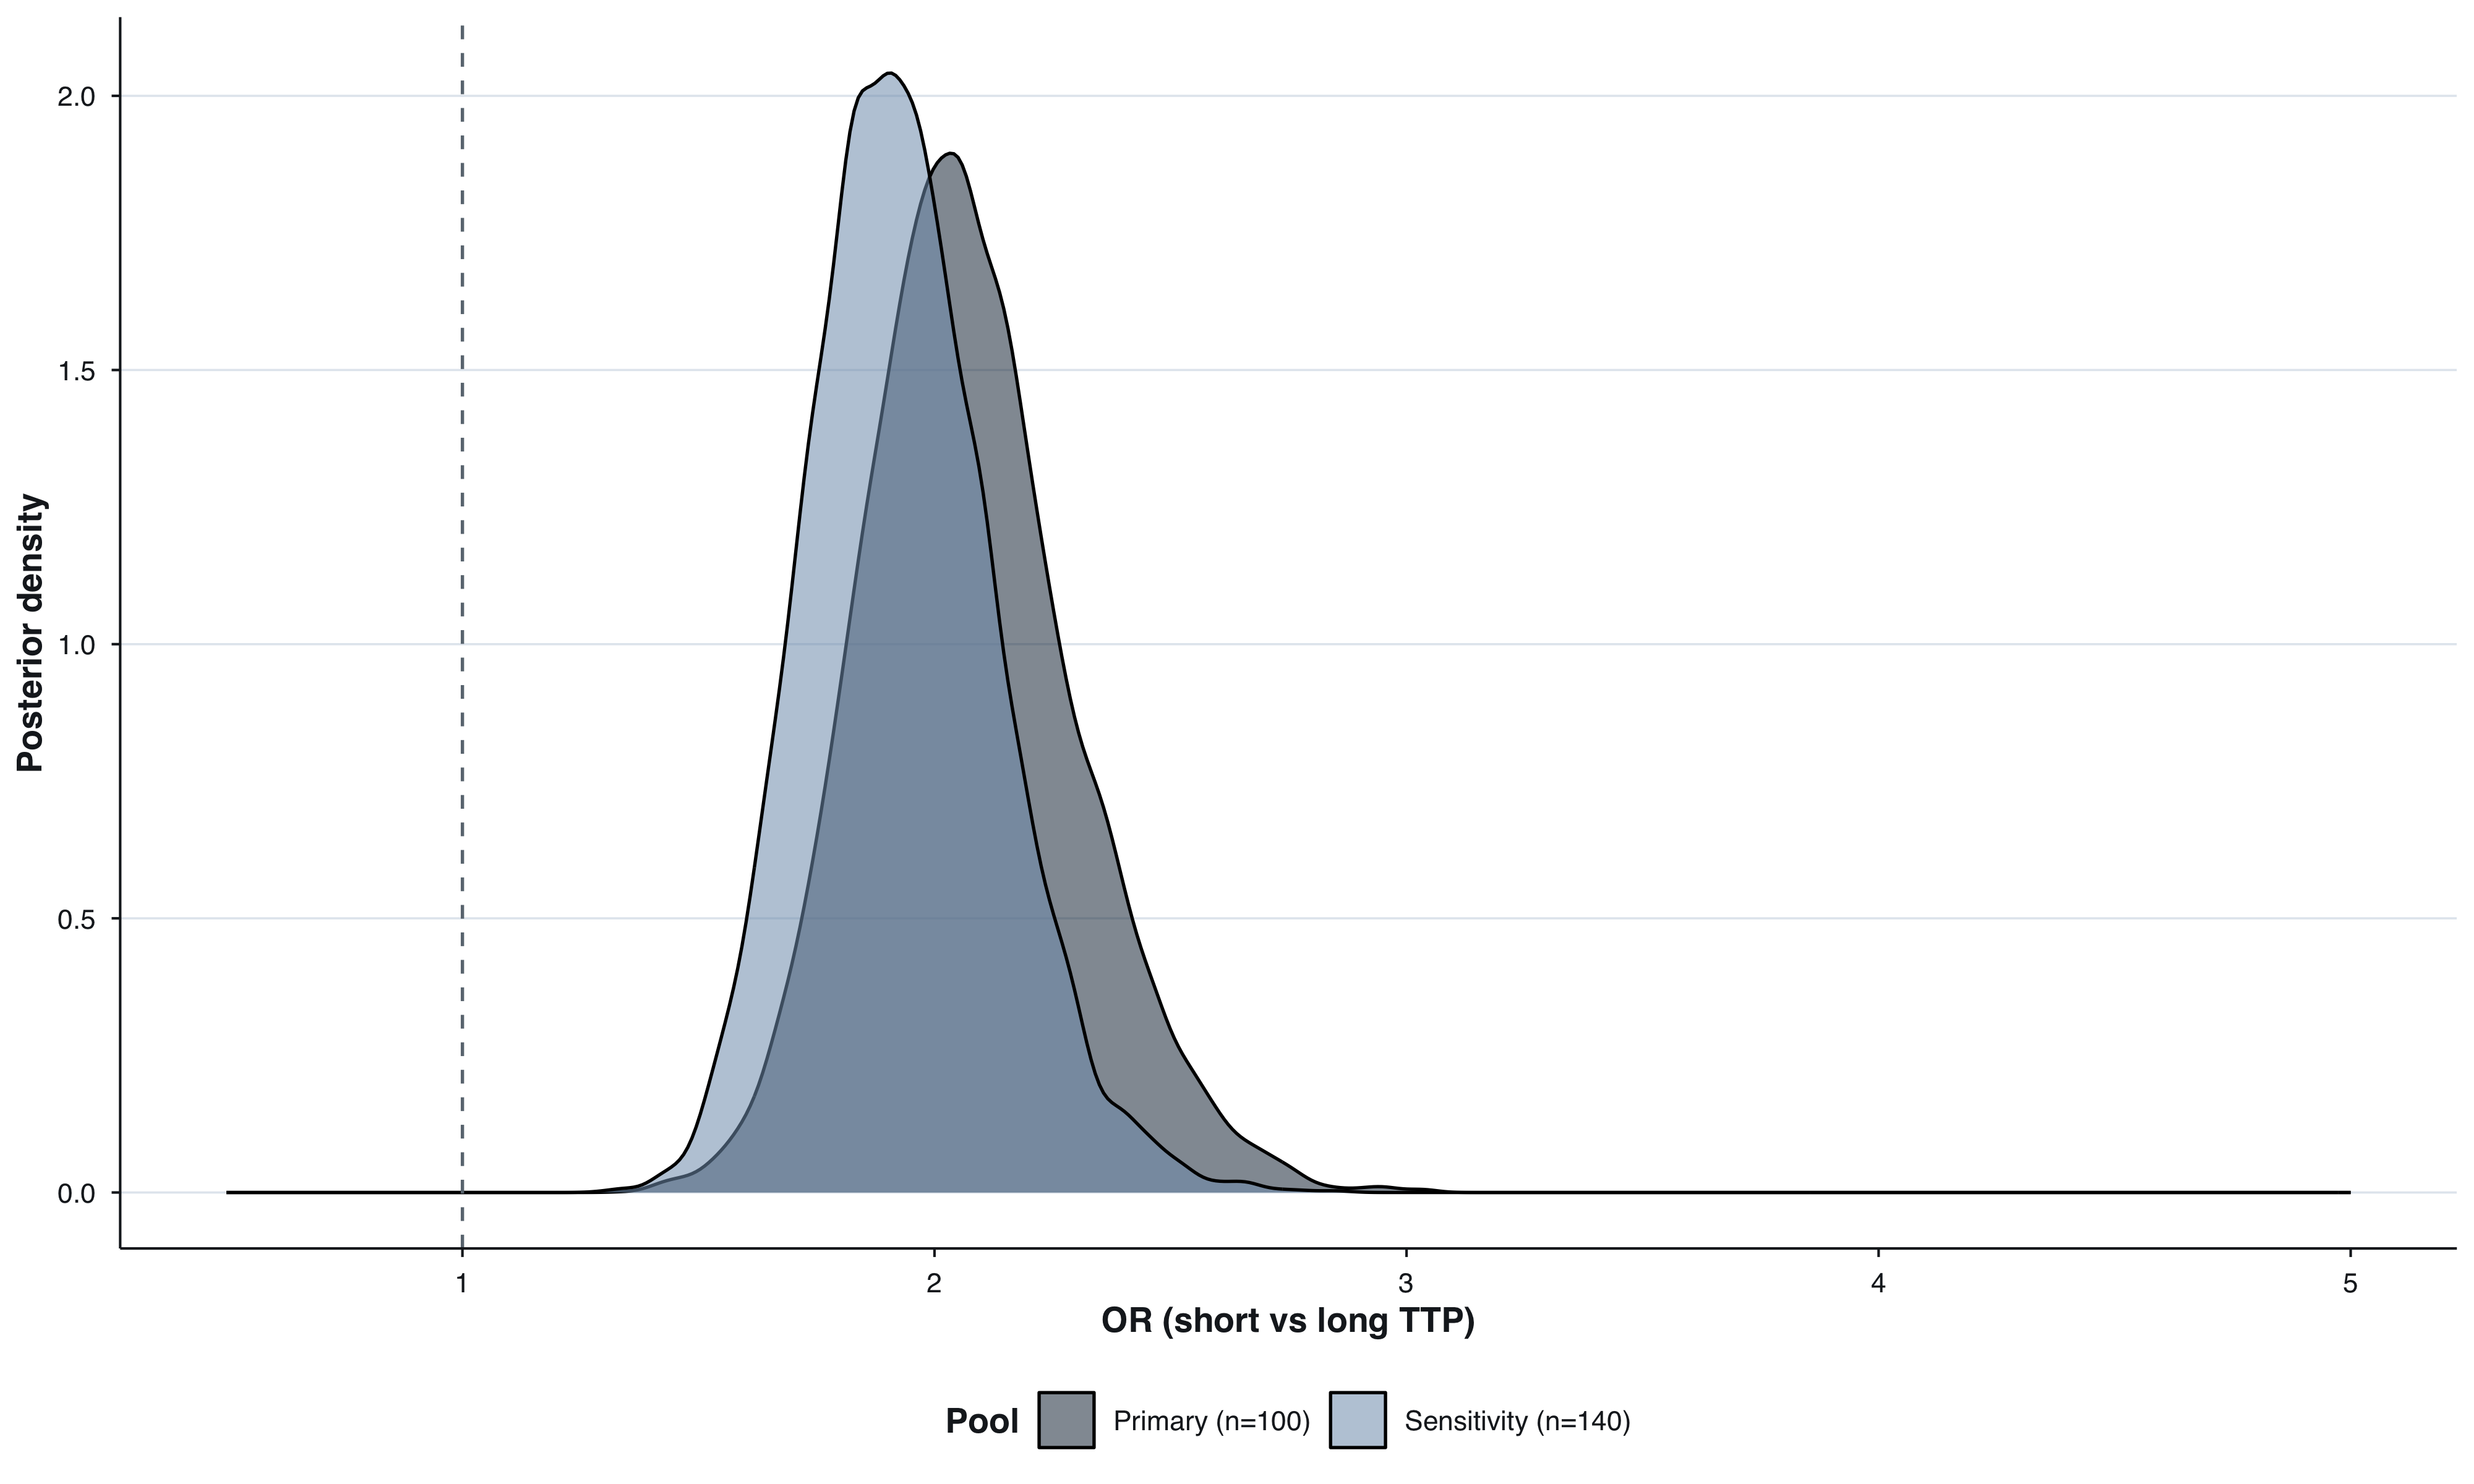
\includegraphics[keepaspectratio]{index_files/figure-latex/notebooks-mortality-analysis-fig-sens-inc-output-1.png}}

}

\caption{\label{fig-sens-inc}Posterior densities of pooled OR ---
primary pool vs sensitivity pool (with inclusive-only studies added).}

\end{figure}%

\textsubscript{Source:
\href{https://lewis-id-lab.github.io/ttp-bacteremia-meta-analysis/notebooks/mortality-analysis-preview.html\#cell-fig-sens-inc}{Time-to-Positivity
and Mortality in Bacteremia}}

\subsection{Clinical failure outcomes}\label{clinical-failure-outcomes}

Outcomes other than mortality were reported far less often
(Table~\ref{tbl-counts}). Persistent bacteremia was the most frequently
reported, with 12 effect sizes from 12 studies, followed by
microbiological clearance (4 effect sizes, 3 studies). No usable effect
sizes were available for relapse (0).

Short TTP was associated with higher odds of persistent bacteremia
(pooled OR 1.74 (95\% CrI, 1.09 to 2.80); Figure~\ref{fig-pb}), with
substantial heterogeneity (median \(I^2\) 69\%). Outcome definitions
were not uniform: on review of the outcome definitions, 6 effect sizes
defined persistent bacteremia by duration of positive cultures, 3
defined it by endocarditis or valve involvement, and 3 used other
definitions. In a meta-regression by definition group,
endocarditis-based definitions had a log odds ratio 0.59 higher than
duration-based definitions (95\% CrI -0.19 to 1.24), which is compatible
with no difference given the small number of effect sizes per group. The
pooled persistent-bacteremia estimate should therefore be interpreted as
an association with a heterogeneous composite of outcomes.

For microbiological clearance, the pooled estimate was too imprecise to
interpret (OR 1.63 (95\% CrI, 0.24 to 9.47)), reflecting only 4 effect
sizes with very large between-study heterogeneity (median \(I^2\) 89\%).

{

\begin{longtable}[]{@{}lll@{}}

\caption{\label{tbl-counts}Available effect sizes per clinical-failure
outcome (strict pool).}

\tabularnewline

\toprule\noalign{}
Outcome & Effect sizes & Unique studies \\
\midrule\noalign{}
\endhead
\bottomrule\noalign{}
\endlastfoot
Persistent bacteremia & 12 & 12 \\
Microbiological clearance & 4 & 3 \\
Relapse & 0 & 0 \\

\end{longtable}

}

\textsubscript{Source:
\href{https://lewis-id-lab.github.io/ttp-bacteremia-meta-analysis/notebooks/clinical_failure-preview.html\#cell-tbl-counts}{TTP
and Clinical Failure Outcomes}}

\begin{figure}[H]

\centering{

\pandocbounded{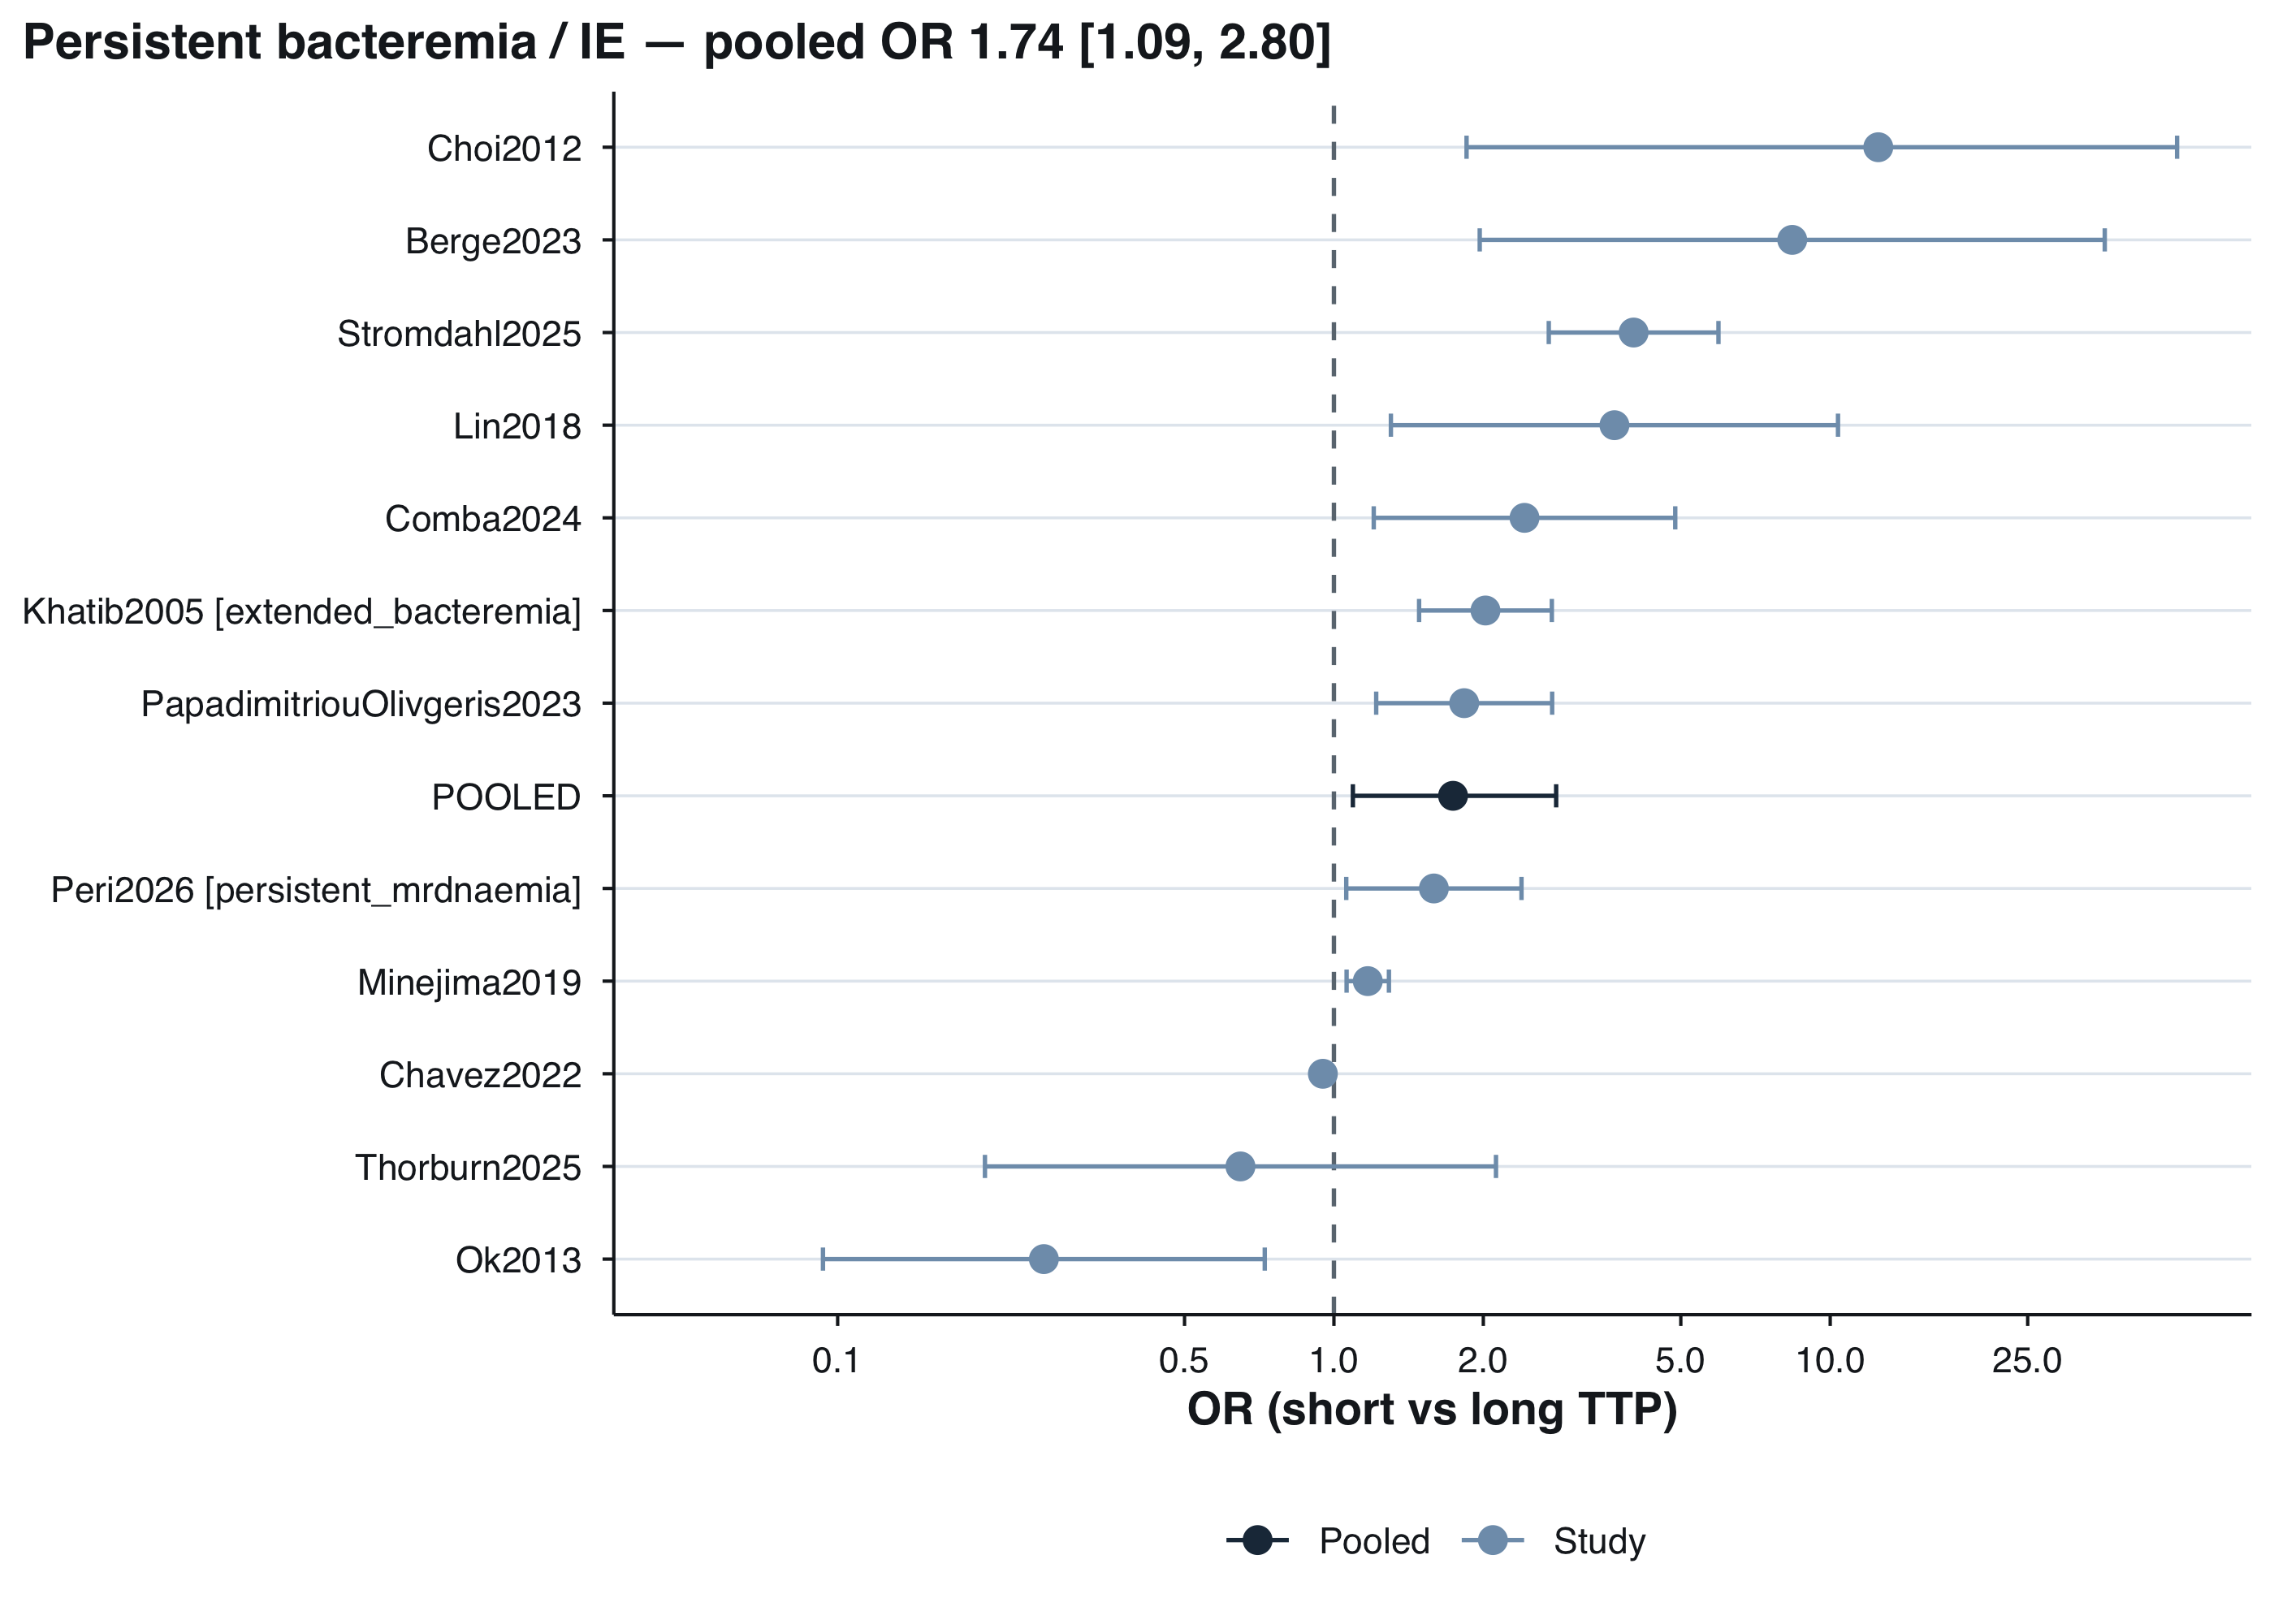
\includegraphics[keepaspectratio]{index_files/figure-latex/notebooks-clinical_failure-fig-pb-output-2.png}}

}

\caption{\label{fig-pb}Forest plot of OR (short vs long TTP) for
persistent bacteremia. NB: many studies coded under
`persistent\_bacteremia' actually report endocarditis (the Codebook's
outcome\_type enum lacks `endocarditis'). Review outcome\_definition in
each row before interpretation.}

\end{figure}%

\textsubscript{Source:
\href{https://lewis-id-lab.github.io/ttp-bacteremia-meta-analysis/notebooks/clinical_failure-preview.html\#cell-fig-pb}{TTP
and Clinical Failure Outcomes}}

\section{Discussion}\label{discussion}

In this Bayesian random-effects meta-analysis, short TTP was associated
with higher mortality in bacteremia (pooled OR 2.06 (95\% CrI, 1.67 to
2.55); 58 studies, 72 effect sizes). The posterior probability that the
association is in the direction of harm was 100.0\%. Between-study
heterogeneity was moderate to substantial (median \(I^2\) 62\%), and the
95\% prediction interval for a new study (0.51 to 8.50) is wide and
includes no association. The pooled estimate is therefore best read as
an average association, not as the effect expected in any particular
setting. Adding studies that met only a more inclusive criterion gave a
similar estimate (OR 1.92 (95\% CrI, 1.58 to 2.35)).

\textbf{Pathogen class.} The association was larger in Gram-negative
bacteremia (OR 2.66 (95\% CrI, 1.72 to 4.06)) than in Gram-positive
bacteremia (OR 1.48 (95\% CrI, 0.85 to 2.58)), for which the credible
interval included 1. The two intervals overlap, so this contrast should
be considered hypothesis-generating rather than confirmed. A plausible
explanation is that TTP in Gram-positive infection, notably \emph{S.
aureus}, is influenced by factors other than burden of disease, such as
the source of infection and the presence of endovascular foci, whereas
in Gram-negative infection it may track inoculum and host response more
directly. This explanation is speculative and was not tested directly
here.

\textbf{Study design and adjustment.} Effect sizes derived from 2×2
tables (OR 2.28 (95\% CrI, 1.74 to 3.05)) were larger than those
back-calculated from reported effect estimates (OR 1.71 (95\% CrI, 1.28
to 2.36)). Meta-regression by data source did not show a clear
difference, and the intervals included zero, so the data are compatible
with either similar or lower adjusted associations. Crude 2×2
comparisons may carry more confounding by severity of illness, source,
or pathogen, in which case the pooled estimate could overstate the
independent prognostic contribution of TTP, but the groups also differ
in other respects.

\textbf{TTP cutpoint.} Studies defined ``short'' TTP using different
thresholds (median cutpoint 12 h), and 30 of 72 mortality effect sizes
did not have a reported cutpoint. In meta-regression among the remaining
effect sizes, the log OR decreased by 0.036 per additional hour of
cutpoint (95\% CrI 0.015 to 0.056), meaning that stricter (shorter)
thresholds were associated with larger odds ratios overall
(Figure~\ref{fig-cutpoint}). This gradient was not robust: it was
attenuated when cutpoints above 24 h were excluded, and it was reversed
within Gram-negative studies. Because thresholds are often chosen post
hoc to maximize discrimination in the study sample, the gradient may
partly reflect optimistic cutpoint selection or differences in pathogen
mix, and it should not be interpreted as validating any single clinical
threshold.

\textbf{Other outcomes.} For persistent bacteremia, short TTP was
associated with higher odds (OR 1.74 (95\% CrI, 1.09 to 2.80)), but
outcome definitions varied widely between studies. Evidence for
microbiological clearance was too sparse and imprecise to interpret (OR
1.63 (95\% CrI, 0.24 to 9.47))
(\href{notebooks/clinical_failure.qmd}{notebook}).

\textbf{Strengths and limitations.} Strengths include a multi-database
search with a May 2026 update, a distinction between strict and
inclusive study pools, a Bayesian framework that yields prediction
intervals and direct probability statements, and a fully reproducible
code base. Limitations are substantial. Most included studies were
retrospective cohorts and risk of bias was rated moderate or worse in
most (76 of 100 studies). Several studies contributed multiple effect
sizes, which we handled with study-level random intercepts but which do
not remove all dependence. The TTP threshold, outcome timing, and
adjustment sets were not standardized, and adjustment status varied
across estimates. Blood culture system, bottle type, transport delay,
and prior antibiotic exposure affect TTP and were incompletely reported,
so residual confounding by measurement conditions is likely. The funnel
plot was asymmetric and Egger's test indicated small-study effects
(Figure~\ref{fig-funnel}, Table~\ref{tbl-egger}). Trim-and-fill reduced
the pooled estimate to OR 1.51, so the primary estimate may overstate
the association, although asymmetry can also arise from heterogeneity
and cutpoint optimization, and these tests do not account for multiple
effect sizes per study. Finally, the meta-analysis is based on aggregate
data, which prevents examination of TTP as a continuous predictor within
patients.

\textbf{Implications.} Short TTP is associated with higher mortality on
average, but heterogeneity, the dependence on cutpoint, and probable
confounding limit its use as a stand-alone prognostic tool. These
results support using TTP as one contextual signal, particularly in
Gram-negative bacteremia, alongside clinical severity and pathogen
identification. Individual-patient-data analyses with standardized TTP
measurement, and prospective validation of pathogen-specific thresholds,
are needed before TTP can be used to guide treatment decisions.

\section*{Funding}\label{funding}
\addcontentsline{toc}{section}{Funding}

No specific funding was received for this study. The authors are
supported by their institutional salaries (University of Padova).
{[}Confirm.{]}

\section*{Conflicts of interest}\label{conflicts-of-interest}
\addcontentsline{toc}{section}{Conflicts of interest}

R.E.L. serves as an Associate Editor at the Journal of Antimicrobial
Chemotherapy. The other author declares no conflicts of interest.
{[}Confirm with all co-authors.{]}

\section*{Data and code availability}\label{data-and-code-availability}
\addcontentsline{toc}{section}{Data and code availability}

The extraction workbook, analysis code, and rendered notebooks are
included in the manuscript project. {[}Insert repository and DOI, for
example an OSF project, once deposited.{]}

\section*{Use of artificial
intelligence}\label{use-of-artificial-intelligence}
\addcontentsline{toc}{section}{Use of artificial intelligence}

A large language model agent was used to assist with full-text screening
and data extraction for the 2026 update, and a second, independent agent
verified the extractions against the source PDFs, as described in the
Methods. {[}State the model name and version, how authors reviewed
outputs, and who is responsible for the final data. Confirm the wording
against ASM's current policy on AI use.{]} Analysis code was written and
run in R and Stan. The authors take responsibility for the content of
the manuscript.

\section*{Acknowledgments}\label{acknowledgments}
\addcontentsline{toc}{section}{Acknowledgments}

{[}None to declare / add acknowledgments.{]}

\section*{References}\label{references}
\addcontentsline{toc}{section}{References}

\protect\phantomsection\label{refs}
\begin{CSLReferences}{0}{1}
\bibitem[\citeproctext]{ref-Sowden2008}
\CSLLeftMargin{1. }%
\CSLRightInline{Sowden D, Anstey C, Faddy M. 2008.
\href{https://doi.org/10.1016/j.jinf.2008.01.005}{{Blood culture time to
positivity as a predictor of mortality in community acquired
Methicillin-susceptible Staphylococcus aureus bacteremia}}. Journal of
Infection 56:295--296.}

\bibitem[\citeproctext]{ref-Kahn2021}
\CSLLeftMargin{2. }%
\CSLRightInline{Kahn F, Resman F, Bergmark S, Filiptsev P, Nilson B,
Gilje P, Rasmussen M. 2021.
\href{https://doi.org/10.1016/j.cmi.2020.11.007}{{Time to blood culture
positivity in Staphylococcus aureus bacteraemia to determine risk of
infective endocarditis}}. Clinical Microbiology and Infection
27:1345.e7--1345.e12.}

\bibitem[\citeproctext]{ref-Stromdahl2025}
\CSLLeftMargin{3. }%
\CSLRightInline{Strömdahl M, Hagman K, Hedman K, Westman A, Hedenstierna
M, Ursing J. 2025. \href{https://doi.org/10.1093/cid/ciae628}{{Time to
Staphylococcus aureus Blood Culture Positivity as a Risk Marker of
Infective Endocarditis: A Retrospective Cohort Study}}. Clinical
Infectious Diseases 80:727--734.}

\bibitem[\citeproctext]{ref-Willmann2013}
\CSLLeftMargin{4. }%
\CSLRightInline{Willmann M, Kuebart I, Vogel W, Flesch I, Markert U,
Marschal M, Schröppel K, Autenrieth IB, Hölzl F, Peter S. 2013.
\href{https://doi.org/10.1016/j.jinf.2013.06.012}{{Time to positivity as
prognostic tool in patients with Pseudomonas aeruginosa bloodstream
infection}}. Journal of Infection 67:416--423.}

\bibitem[\citeproctext]{ref-Tang2017}
\CSLLeftMargin{5. }%
\CSLRightInline{Tang P-C, Lee C-C, Li C-W, Li M-C, Ko W-C, Lee N-Y.
2017.
\href{https://doi.org/10.1016/j.jmii.2015.08.014}{{Time-to-positivity of
blood culture: An independent prognostic factor of monomicrobial
Pseudomonas aeruginosa bacteremia}}. Journal of Microbiology, Immunology
and Infection 50:486--493.}

\bibitem[\citeproctext]{ref-Martinez2006}
\CSLLeftMargin{6. }%
\CSLRightInline{Martínez JA, Soto S, Fabrega A, Almela M, Mensa J,
Soriano A, Marco F, Jimenez De Anta MT, Vila J. 2006.
\href{https://doi.org/10.1128/JCM.44.4.1468-1474.2006}{{Relationship of
phylogenetic background, biofilm production, and time to detection of
growth in blood culture vials with clinical variables and prognosis
associated with Escherichia coli bacteremia}}. Journal of Clinical
Microbiology 44:1468--1474.}

\bibitem[\citeproctext]{ref-Keighley2023}
\CSLLeftMargin{7. }%
\CSLRightInline{Keighley C, Pope AL, Marriott D, Chen SC-A, Slavin MA.
2023. \href{https://doi.org/10.1093/mmy/myad028}{{Time-to-positivity in
bloodstream infection for Candida species as a prognostic marker for
mortality}}. Medical Mycology 61.}

\bibitem[\citeproctext]{ref-PuertaAlcalde2019}
\CSLLeftMargin{8. }%
\CSLRightInline{Puerta-Alcalde P, Cardozo C, Suárez-Lledó M,
Rodríguez-Núñez O, Morata L, Fehér C, Marco F, Del Río A, Martínez JA,
Mensa J, Rovira M, Esteve J, Soriano A, Garcia-Vidal C. 2019.
\href{https://doi.org/10.1016/j.cmi.2018.07.026}{{Current
time-to-positivity of blood cultures in febrile neutropenia: a tool to
be used in stewardship de-escalation strategies}}. Clinical Microbiology
and Infection 25:447--453.}

\end{CSLReferences}

\section*{Supplementary appendix: model specification and
diagnostics}\label{supplementary-appendix-model-specification-and-diagnostics}
\addcontentsline{toc}{section}{Supplementary appendix: model
specification and diagnostics}

\subsection*{Model specification}\label{model-specification}
\addcontentsline{toc}{subsection}{Model specification}

All pooled and moderator models were Bayesian random-effects models
fitted with \texttt{brms}:
\(y_i \mid \mathrm{SE}_i \sim \mathcal{N}(\mu + u_s,\ \mathrm{SE}_i^2)\)
with study-level random intercepts \(u_s \sim \mathcal{N}(0, \tau^2)\),
where \(y_i\) is the log odds ratio for effect size \(i\) and
\(\mathrm{SE}_i\) its standard error. Priors were
\(\mu \sim \mathcal{N}(0, 1)\),
\(\tau \sim \text{Half-Cauchy}(0, 0.5)\), and \(\mathcal{N}(0, 0.5)\)
for moderator coefficients. Each model used 4 chains of 4,000 iterations
(1,000 warm-up; 12,000 post-warm-up draws),
\texttt{adapt\_delta\ =\ 0.99}, and \texttt{max\_treedepth\ =\ 12}. The
persistent bacteremia and microbiological clearance models were fitted
with the CmdStan backend and all others with rstan. Convergence was
judged by \(\hat{R} < 1.01\), bulk and tail effective sample sizes,
divergent transitions, and visual inspection of trace and rank plots.
Code is in \texttt{R/02\_fit\_models.R} and the notebooks.

\subsection*{Convergence across all fitted
models}\label{convergence-across-all-fitted-models}
\addcontentsline{toc}{subsection}{Convergence across all fitted models}

{

\begin{longtable}[]{@{}
  >{\raggedright\arraybackslash}p{(\linewidth - 10\tabcolsep) * \real{0.2617}}
  >{\raggedright\arraybackslash}p{(\linewidth - 10\tabcolsep) * \real{0.0935}}
  >{\raggedright\arraybackslash}p{(\linewidth - 10\tabcolsep) * \real{0.1215}}
  >{\raggedright\arraybackslash}p{(\linewidth - 10\tabcolsep) * \real{0.1215}}
  >{\raggedleft\arraybackslash}p{(\linewidth - 10\tabcolsep) * \real{0.2056}}
  >{\raggedleft\arraybackslash}p{(\linewidth - 10\tabcolsep) * \real{0.1963}}@{}}

\caption{\label{tbl-conv-all}Convergence diagnostics for every fitted
model. Parameters are population-level effects and the between-study SD;
study-level random effects are not summarized.}

\tabularnewline

\toprule\noalign{}
\begin{minipage}[b]{\linewidth}\raggedright
Model
\end{minipage} & \begin{minipage}[b]{\linewidth}\raggedright
Max R-hat
\end{minipage} & \begin{minipage}[b]{\linewidth}\raggedright
Min bulk ESS
\end{minipage} & \begin{minipage}[b]{\linewidth}\raggedright
Min tail ESS
\end{minipage} & \begin{minipage}[b]{\linewidth}\raggedleft
Divergent transitions
\end{minipage} & \begin{minipage}[b]{\linewidth}\raggedleft
Treedepth limit hits
\end{minipage} \\
\midrule\noalign{}
\endhead
\bottomrule\noalign{}
\endlastfoot
fit\_2x2 & 1.001 & 3334 & 4906 & 0 & 0 \\
fit\_adjustment & 1.004 & 1702 & 2781 & 0 & 0 \\
fit\_base & 1.003 & 1429 & 2831 & 0 & 0 \\
fit\_clr & 1.000 & 2748 & 3191 & 2 & 0 \\
fit\_cutpoint\_le24 & 1.001 & 3806 & 5910 & 0 & 0 \\
fit\_cutpoint & 1.001 & 3854 & 5342 & 0 & 0 \\
fit\_es\_source & 1.003 & 1978 & 3585 & 0 & 0 \\
fit\_fungal & 1.001 & 3388 & 4296 & 8 & 0 \\
fit\_gneg\_cutpoint & 1.000 & 3219 & 3938 & 0 & 0 \\
fit\_gpos\_cutpoint\_sens & 1.001 & 2110 & 3010 & 0 & 0 \\
fit\_gpos\_cutpoint & 1.001 & 2304 & 3438 & 1 & 0 \\
fit\_gram\_neg & 1.001 & 2557 & 3765 & 0 & 0 \\
fit\_gram\_pos & 1.002 & 2650 & 4142 & 0 & 0 \\
fit\_metareg & 1.003 & 3164 & 4357 & 0 & 0 \\
fit\_mixed\_source & 1.002 & 2246 & 3595 & 0 & 0 \\
fit\_pb\_defgroup & 1.001 & 2866 & 4597 & 0 & 0 \\
fit\_pb & 1.002 & 2135 & 3478 & 0 & 0 \\
fit\_reported & 1.003 & 1958 & 3610 & 0 & 0 \\
fit\_src\_binary & 1.001 & 2795 & 5091 & 0 & 0 \\
fit\_year & 1.003 & 1572 & 3301 & 0 & 0 \\
fit\_base (sensitivity pool) & 1.002 & 1789 & 2906 & 0 & 0 \\

\end{longtable}

}

\textsubscript{Source:
\href{https://lewis-id-lab.github.io/ttp-bacteremia-meta-analysis/index-preview.html}{Article
Notebook}}

The maximum \(\hat{R}\) across models was 1.004 and the minimum bulk ESS
was 1,429. Divergent transitions occurred in 11 post-warm-up draws in
total, confined to these models: fit\_clr, fit\_fungal,
fit\_gpos\_cutpoint. Estimates from models with divergent transitions,
which have few effect sizes, should be interpreted cautiously.

\subsection*{Primary pool: pooled
model}\label{primary-pool-pooled-model}
\addcontentsline{toc}{subsection}{Primary pool: pooled model}

{

\begin{longtable}[]{@{}lll@{}}

\caption{\label{tbl-diag}Convergence diagnostics for the primary pooled
model.}

\tabularnewline

\toprule\noalign{}
Parameter & R̂ & ESS\_bulk \\
\midrule\noalign{}
\endhead
\bottomrule\noalign{}
\endlastfoot
b\_Intercept & 1.003 & 1429 \\
sd\_study\_id\_\_Intercept & 1.002 & 2043 \\
sigma & NA & NA \\
Intercept & 1.003 & 1429 \\
r\_study\_id{[}Alvarez2012,Intercept{]} & 1.001 & 10557 \\
r\_study\_id{[}Bae2021,Intercept{]} & 1.000 & 12229 \\
r\_study\_id{[}Balaji2024,Intercept{]} & 1.002 & 2836 \\
r\_study\_id{[}Barr2022,Intercept{]} & 1.000 & 11548 \\
r\_study\_id{[}Blackberg2022,Intercept{]} & 1.001 & 11388 \\
r\_study\_id{[}Blackberg2023,Intercept{]} & 1.001 & 9980 \\
r\_study\_id{[}Bo2011,Intercept{]} & 1.000 & 7848 \\
r\_study\_id{[}Chavez2022,Intercept{]} & 1.003 & 1426 \\
r\_study\_id{[}Chen2018,Intercept{]} & 1.000 & 6414 \\
r\_study\_id{[}Chen2020,Intercept{]} & 1.000 & 14148 \\
r\_study\_id{[}Chen2023,Intercept{]} & 1.000 & 13576 \\
r\_study\_id{[}Cheng2022,Intercept{]} & 1.000 & 13904 \\
r\_study\_id{[}Cilloniz2017,Intercept{]} & 1.000 & 7851 \\
r\_study\_id{[}Deguchi2024,Intercept{]} & 1.000 & 12353 \\
r\_study\_id{[}Fenoll2022,Intercept{]} & 1.000 & 10865 \\
r\_study\_id{[}Hamilton2021,Intercept{]} & 1.003 & 1432 \\
r\_study\_id{[}Hou2023,Intercept{]} & 1.001 & 7382 \\
r\_study\_id{[}Hsieh2022,Intercept{]} & 1.001 & 3480 \\
r\_study\_id{[}IrigoyenSierakowski2024,Intercept{]} & 1.000 & 16462 \\
r\_study\_id{[}Jayabalakrishnan2022,Intercept{]} & 1.000 & 16215 \\
r\_study\_id{[}Ji2020,Intercept{]} & 1.000 & 6152 \\
r\_study\_id{[}Kahn2021,Intercept{]} & 1.000 & 6419 \\
r\_study\_id{[}Keighley2023,Intercept{]} & 1.000 & 16962 \\
r\_study\_id{[}Kim2010,Intercept{]} & 1.001 & 5819 \\
r\_study\_id{[}Kim2013,Intercept{]} & 1.000 & 9157 \\
r\_study\_id{[}Laupland2022,Intercept{]} & 1.002 & 1610 \\
r\_study\_id{[}Laupland2024,Intercept{]} & 1.003 & 1478 \\
r\_study\_id{[}Liao2009,Intercept{]} & 1.000 & 8344 \\
r\_study\_id{[}Lin2016,Intercept{]} & 1.000 & 13218 \\
r\_study\_id{[}Marco2025,Intercept{]} & 1.001 & 4825 \\
r\_study\_id{[}Marra2006,Intercept{]} & 1.000 & 13785 \\
r\_study\_id{[}Minejima2019,Intercept{]} & 1.001 & 8153 \\
r\_study\_id{[}Nunes2013,Intercept{]} & 1.000 & 13928 \\
r\_study\_id{[}Ok2013,Intercept{]} & 1.000 & 12816 \\
r\_study\_id{[}Palmer2013,Intercept{]} & 1.001 & 15976 \\
r\_study\_id{[}PapadimitriouOlivgeris2023,Intercept{]} & 1.000 & 5065 \\
r\_study\_id{[}Paquette2021,Intercept{]} & 1.003 & 1576 \\
r\_study\_id{[}Peralta2007,Intercept{]} & 1.000 & 10735 \\
r\_study\_id{[}PerezRodriguez2024,Intercept{]} & 1.000 & 10843 \\
r\_study\_id{[}Prinsloo2023,Intercept{]} & 1.000 & 9664 \\
r\_study\_id{[}PuertaAlcalde2019,Intercept{]} & 1.001 & 6856 \\
r\_study\_id{[}Recio2020,Intercept{]} & 1.003 & 1490 \\
r\_study\_id{[}Rojas2013,Intercept{]} & 1.001 & 14005 \\
r\_study\_id{[}Rolo2022,Intercept{]} & 1.000 & 8569 \\
r\_study\_id{[}Sachu2024,Intercept{]} & 1.000 & 11112 \\
r\_study\_id{[}Savithri2011,Intercept{]} & 1.000 & 16329 \\
r\_study\_id{[}Simeon2019,Intercept{]} & 1.001 & 5714 \\
r\_study\_id{[}Sowden2008,Intercept{]} & 1.000 & 12698 \\
r\_study\_id{[}Takahashi2022,Intercept{]} & 1.000 & 13238 \\
r\_study\_id{[}Tang2017,Intercept{]} & 1.001 & 7028 \\
r\_study\_id{[}Taur2010,Intercept{]} & 1.003 & 1440 \\
r\_study\_id{[}Tsai2025,Intercept{]} & 1.003 & 1462 \\
r\_study\_id{[}Turkeltaub2024,Intercept{]} & 1.000 & 14546 \\
r\_study\_id{[}Willmann2013,Intercept{]} & 1.000 & 12819 \\
r\_study\_id{[}Zhang2016,Intercept{]} & 1.000 & 7888 \\
r\_study\_id{[}Zhang2020,Intercept{]} & 1.000 & 9920 \\
r\_study\_id{[}Zhang2021,Intercept{]} & 1.001 & 7441 \\
r\_study\_id{[}Zouggari2022,Intercept{]} & 1.000 & 10868 \\

\end{longtable}

}

\textsubscript{Source:
\href{https://lewis-id-lab.github.io/ttp-bacteremia-meta-analysis/notebooks/mortality-analysis-preview.html\#cell-tbl-diag}{Time-to-Positivity
and Mortality in Bacteremia}}

\begin{figure}[H]

\centering{

\pandocbounded{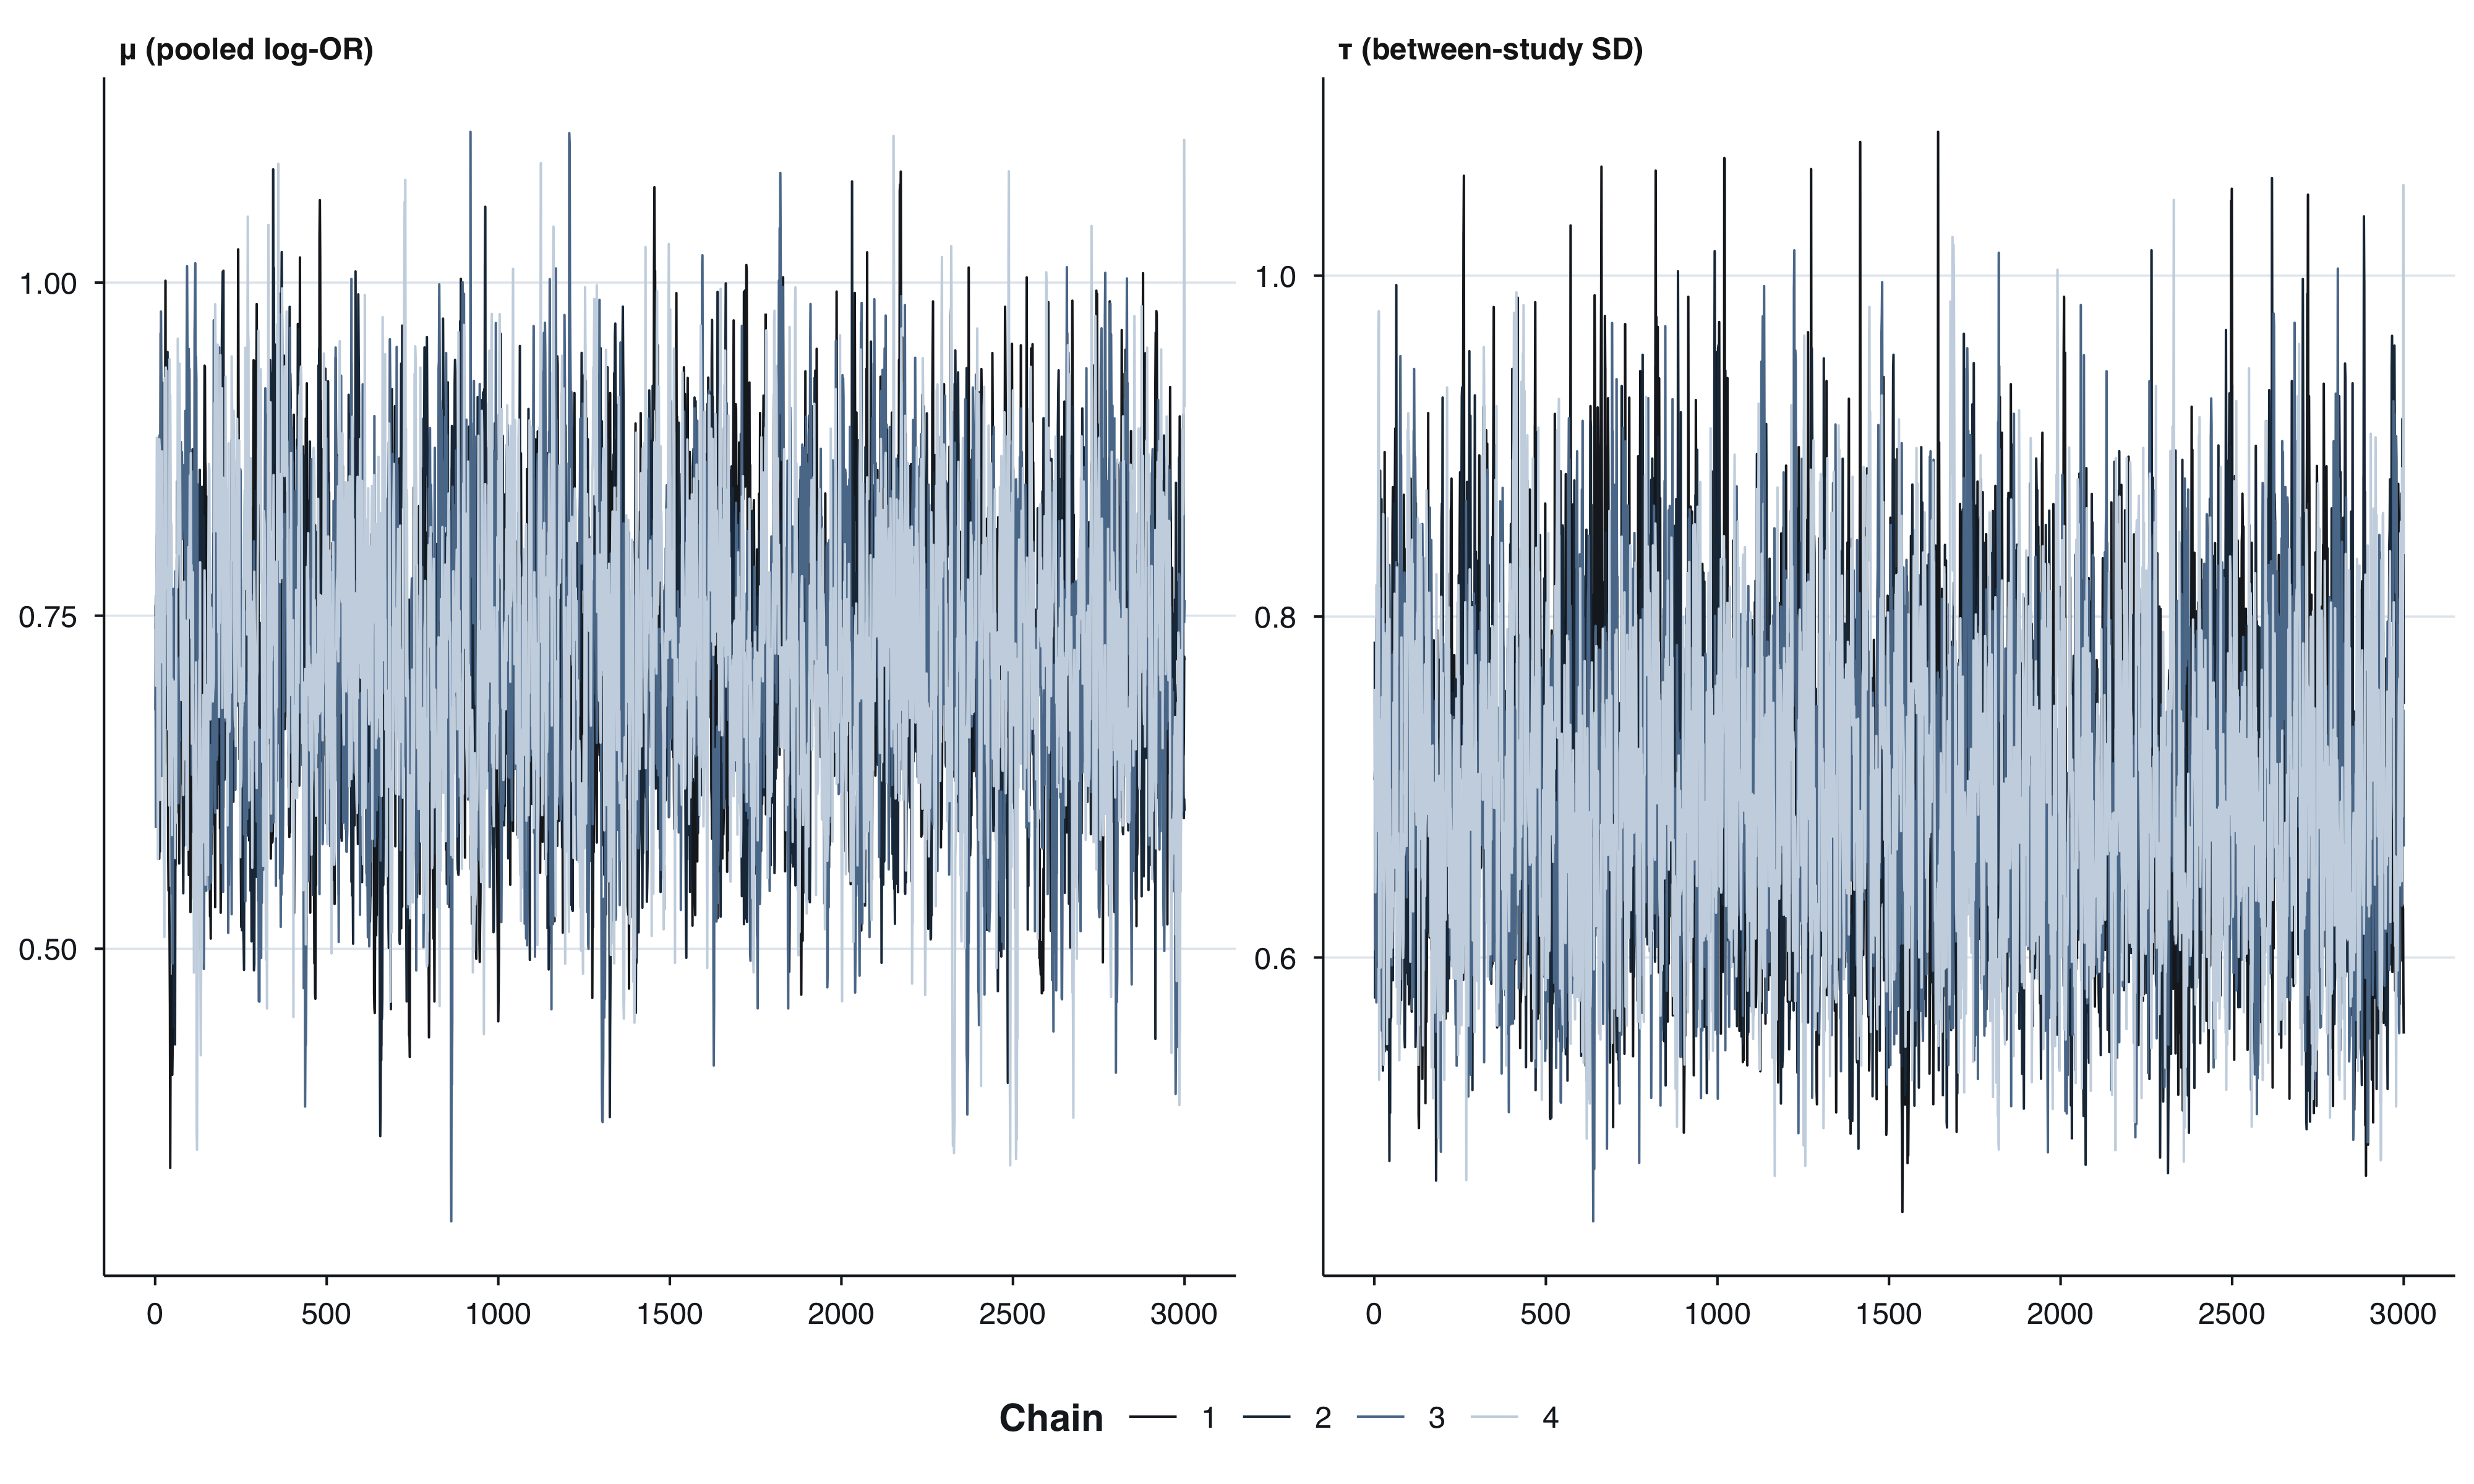
\includegraphics[keepaspectratio]{index_files/figure-latex/notebooks-mortality-analysis-fig-trace-output-1.png}}

}

\caption{\label{fig-trace}Trace plots for key parameters of the primary
pooled model. Well-mixed chains (caterpillar appearance) indicate good
convergence.}

\end{figure}%

\textsubscript{Source:
\href{https://lewis-id-lab.github.io/ttp-bacteremia-meta-analysis/notebooks/mortality-analysis-preview.html\#cell-fig-trace}{Time-to-Positivity
and Mortality in Bacteremia}}

\begin{figure}[H]

\centering{

\pandocbounded{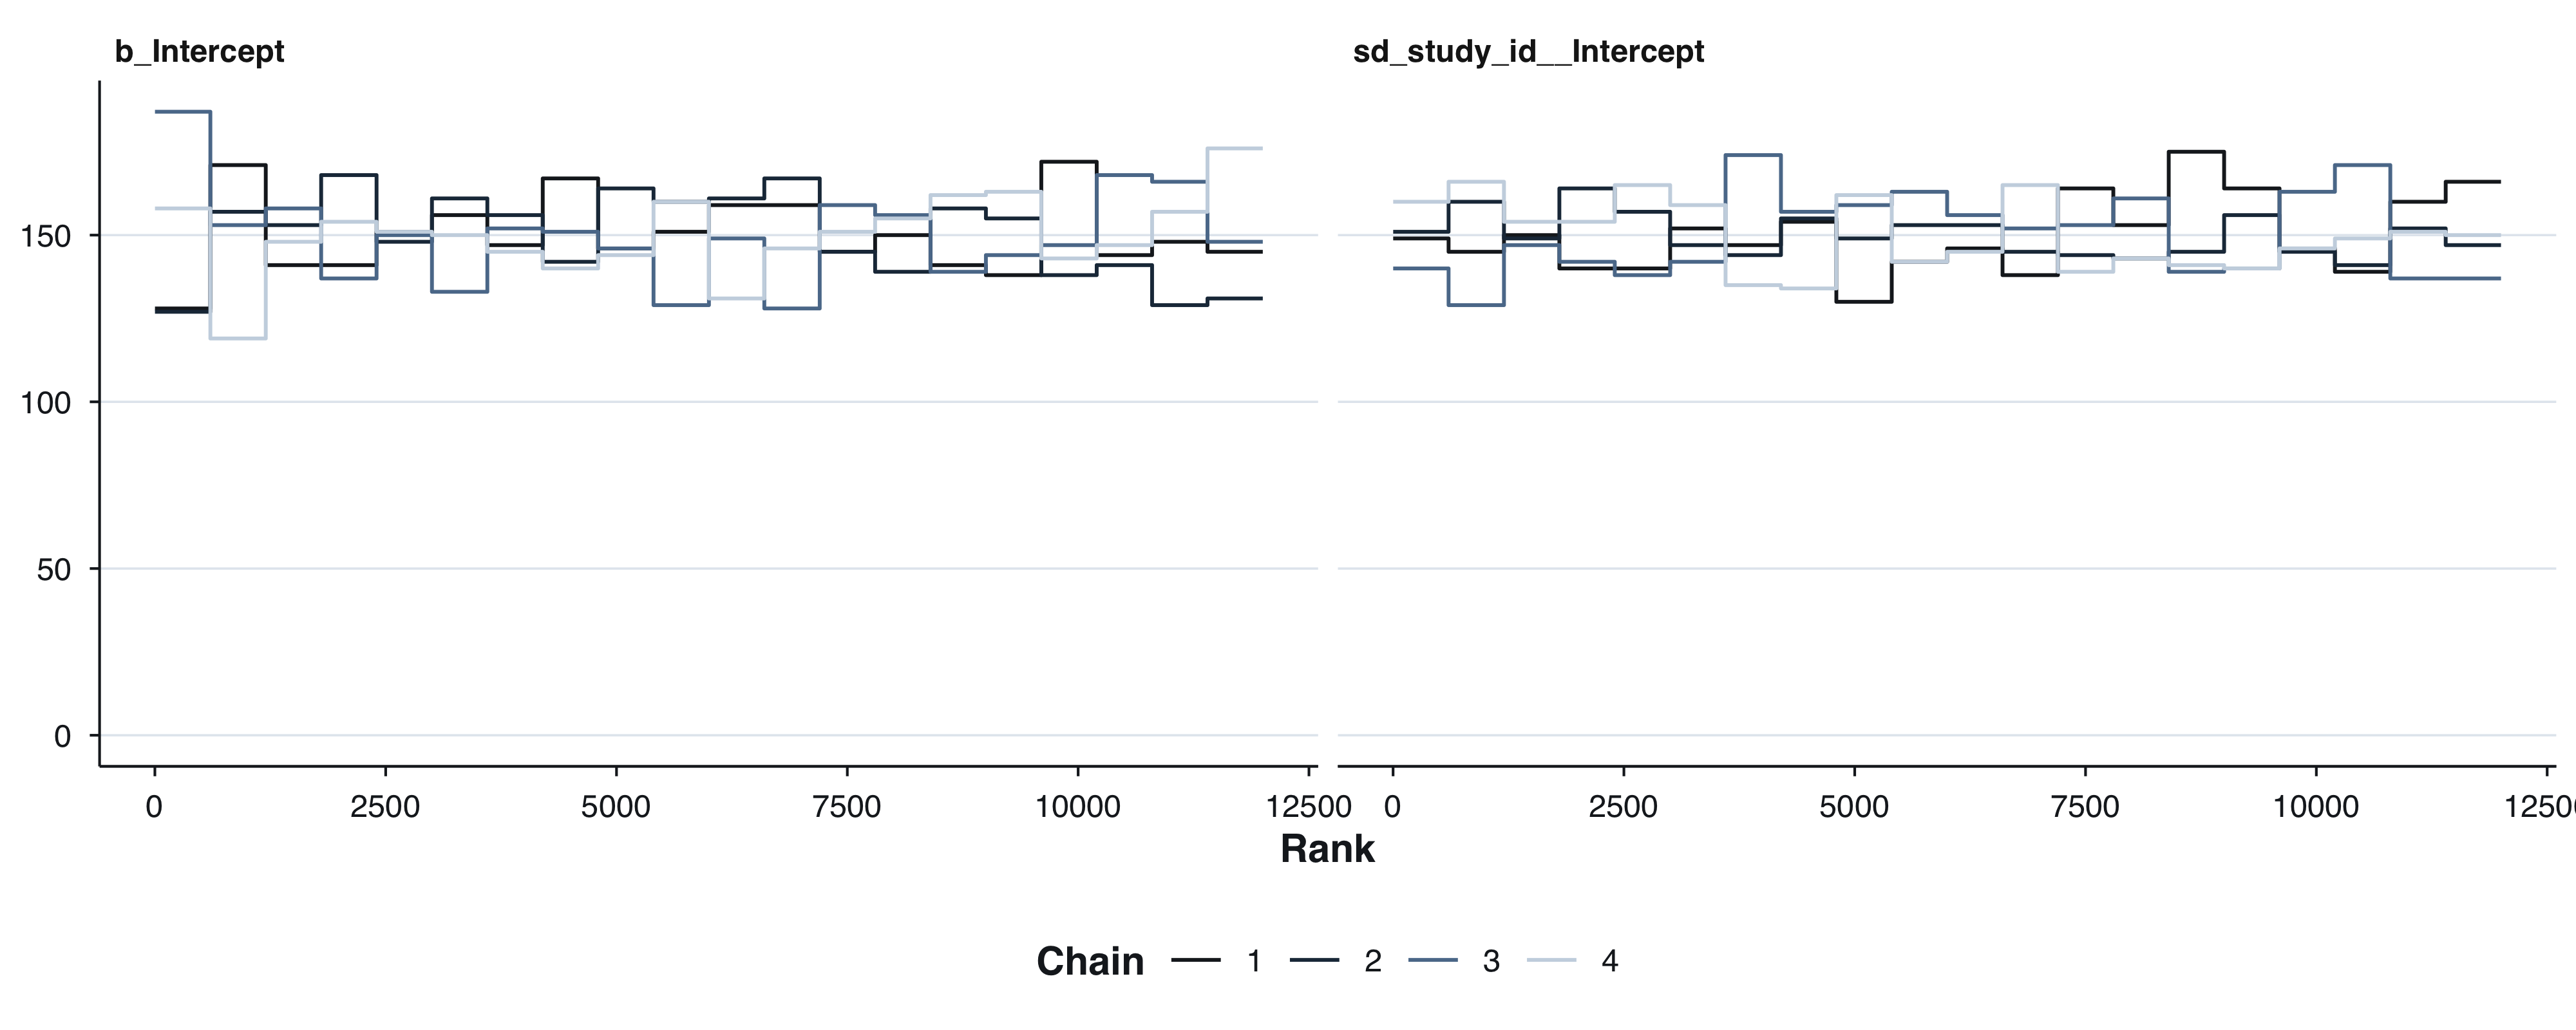
\includegraphics[keepaspectratio]{index_files/figure-latex/notebooks-mortality-analysis-fig-rank-output-1.png}}

}

\caption{\label{fig-rank}Rank histograms for key parameters. Uniform
bars across all chains indicate no chain-mixing issues.}

\end{figure}%

\textsubscript{Source:
\href{https://lewis-id-lab.github.io/ttp-bacteremia-meta-analysis/notebooks/mortality-analysis-preview.html\#cell-fig-rank}{Time-to-Positivity
and Mortality in Bacteremia}}

\begin{figure}[H]

\centering{

\pandocbounded{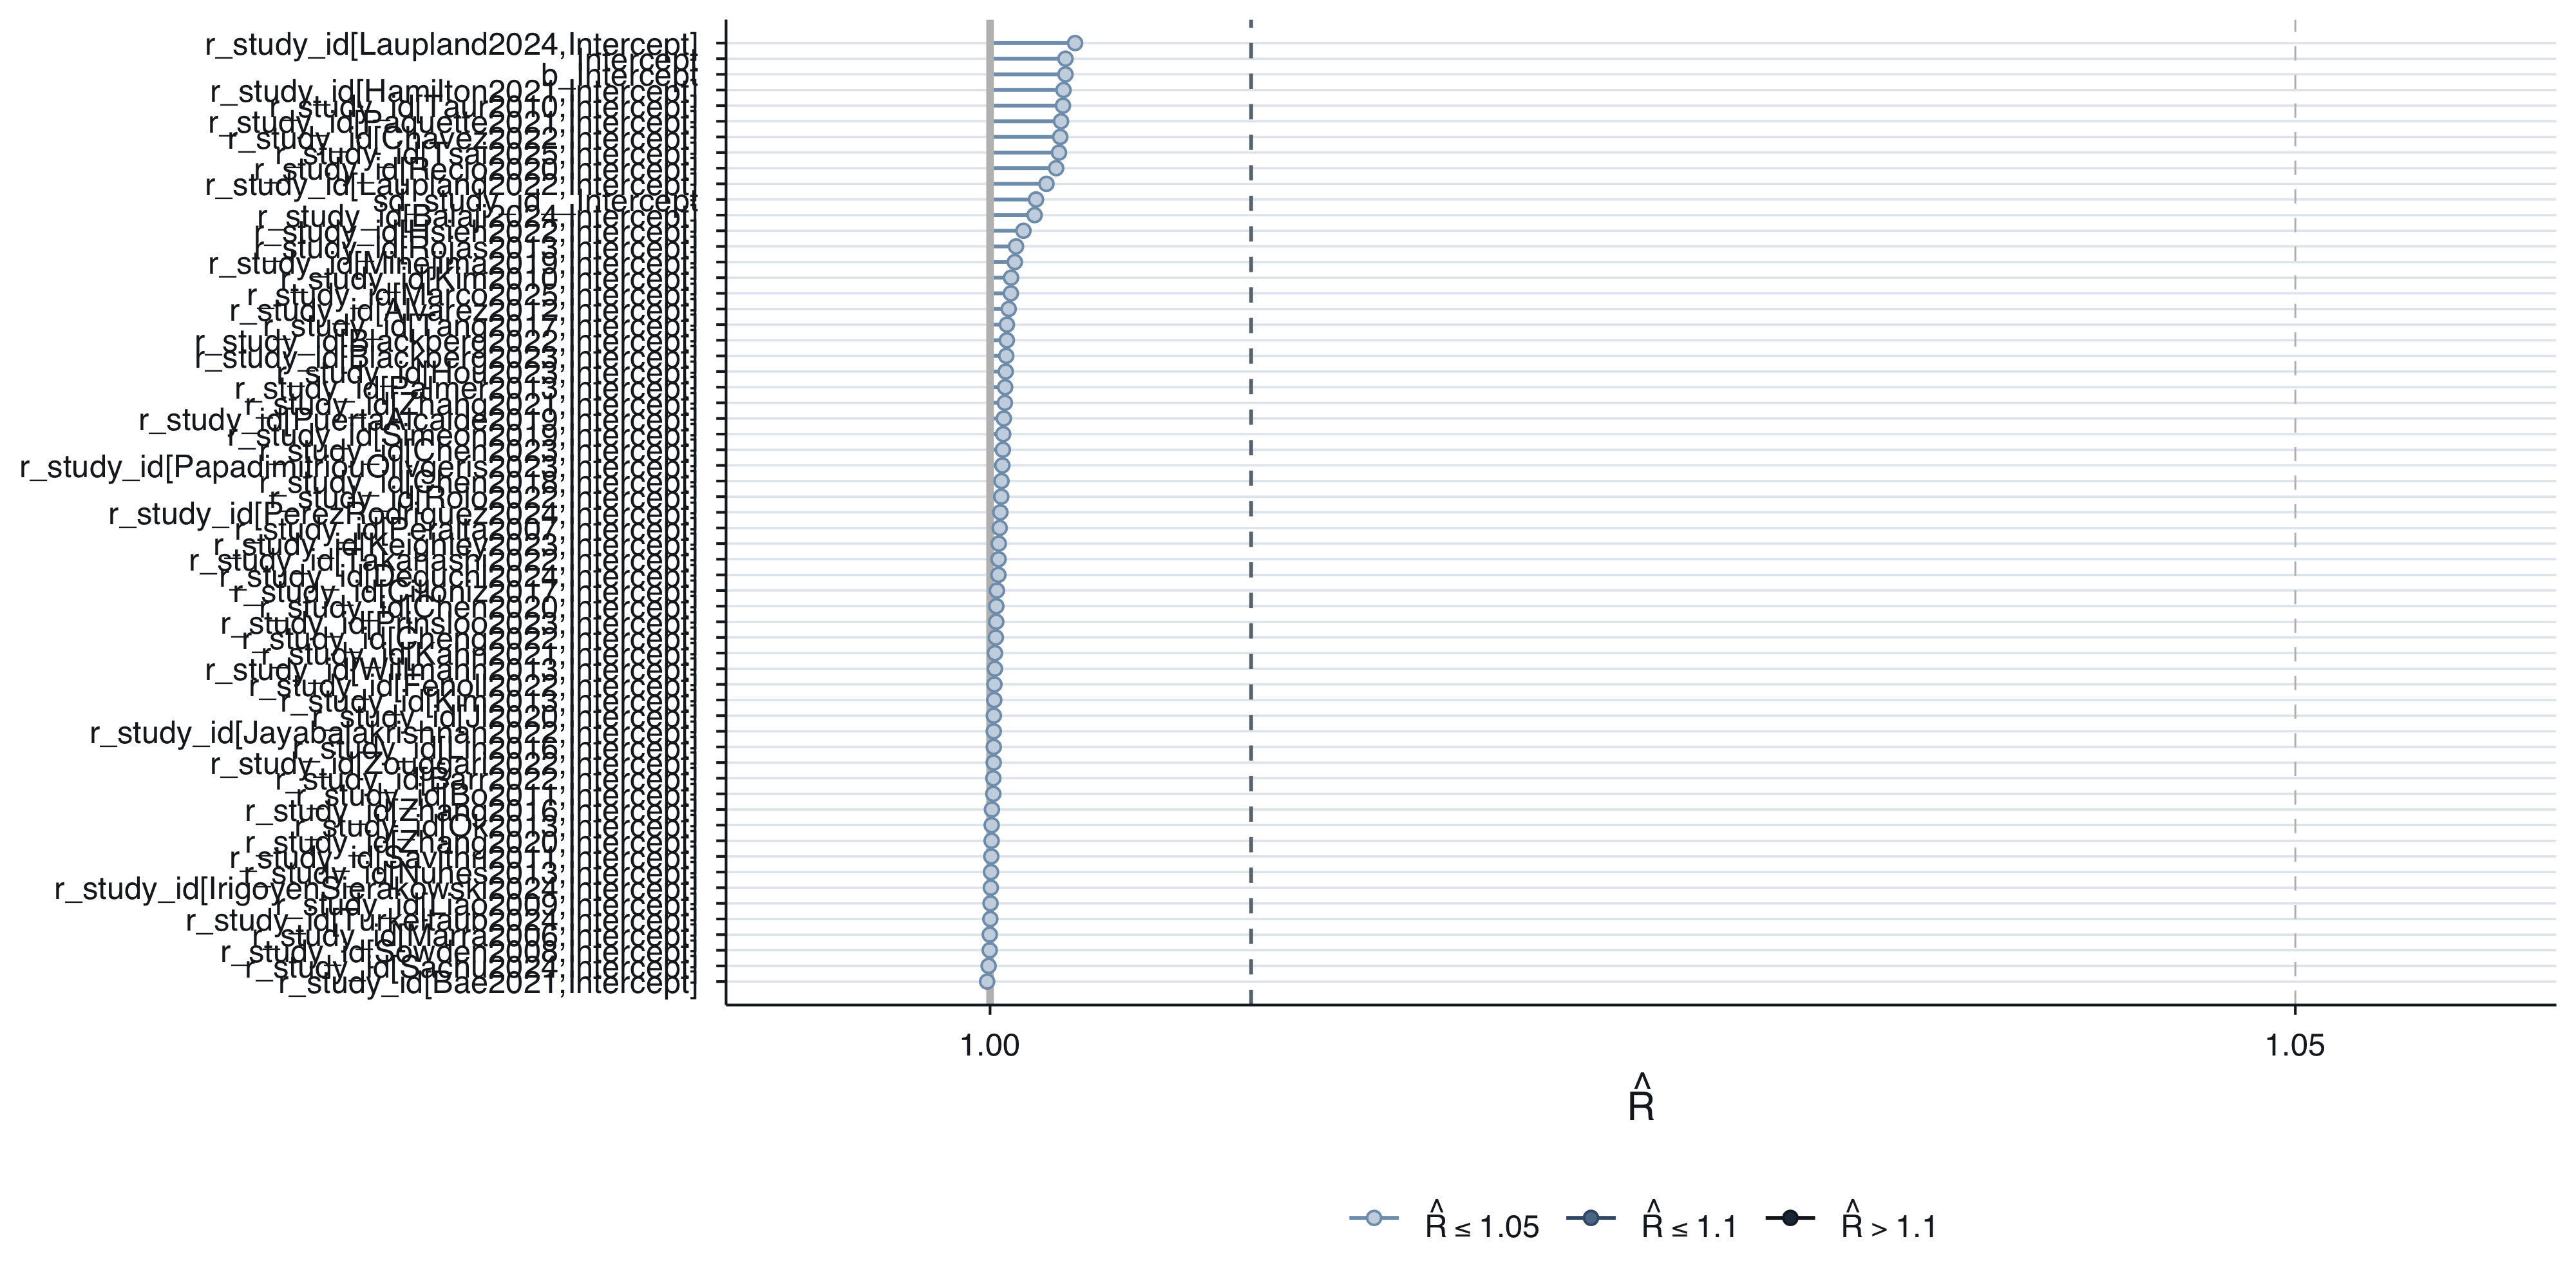
\includegraphics[keepaspectratio]{index_files/figure-latex/notebooks-mortality-analysis-fig-rhat-output-2.png}}

}

\caption{\label{fig-rhat}R̂ dot plot for all parameters of the primary
pooled model. All values should fall below 1.01 (dashed line).}

\end{figure}%

\textsubscript{Source:
\href{https://lewis-id-lab.github.io/ttp-bacteremia-meta-analysis/notebooks/mortality-analysis-preview.html\#cell-fig-rhat}{Time-to-Positivity
and Mortality in Bacteremia}}

\subsection*{Sensitivity pool: pooled
model}\label{sensitivity-pool-pooled-model}
\addcontentsline{toc}{subsection}{Sensitivity pool: pooled model}

\begin{figure}[H]

\centering{

\pandocbounded{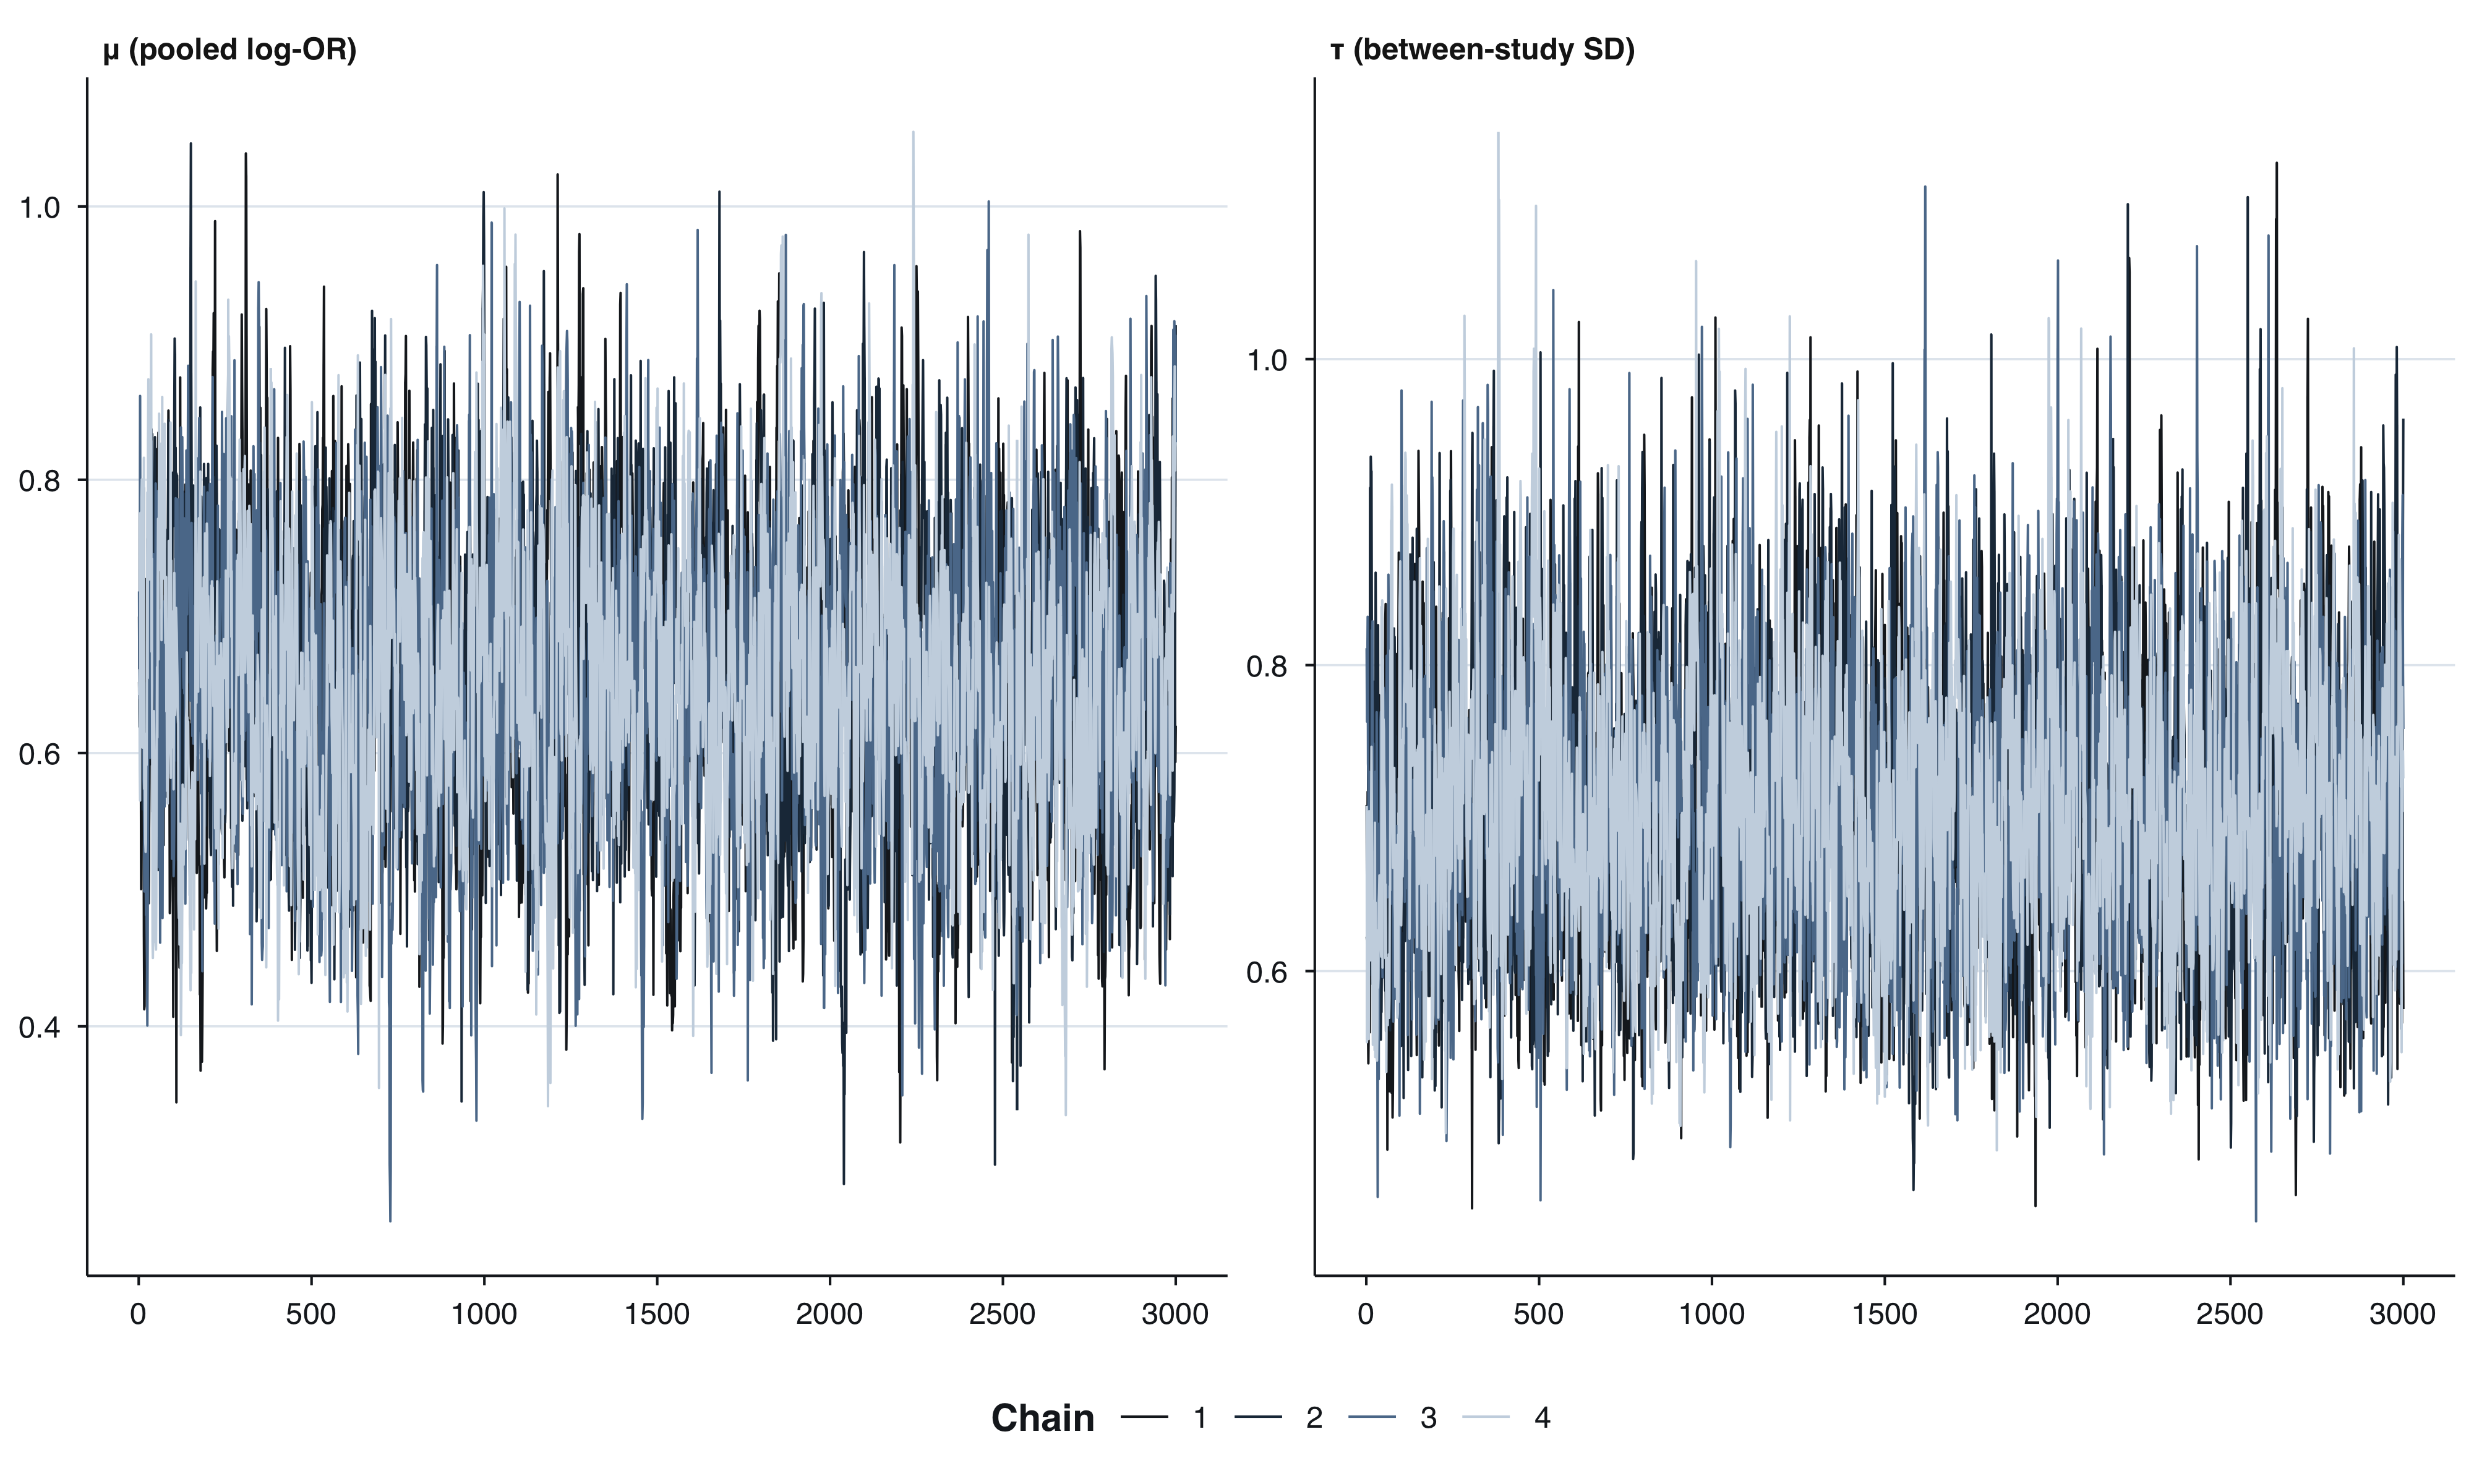
\includegraphics[keepaspectratio]{index_files/figure-latex/notebooks-mortality-analysis-fig-trace-sens-output-1.png}}

}

\caption{\label{fig-trace-sens}Trace plots for key parameters of the
sensitivity (n=140) model.}

\end{figure}%

\textsubscript{Source:
\href{https://lewis-id-lab.github.io/ttp-bacteremia-meta-analysis/notebooks/mortality-analysis-preview.html\#cell-fig-trace-sens}{Time-to-Positivity
and Mortality in Bacteremia}}

\begin{figure}[H]

\centering{

\pandocbounded{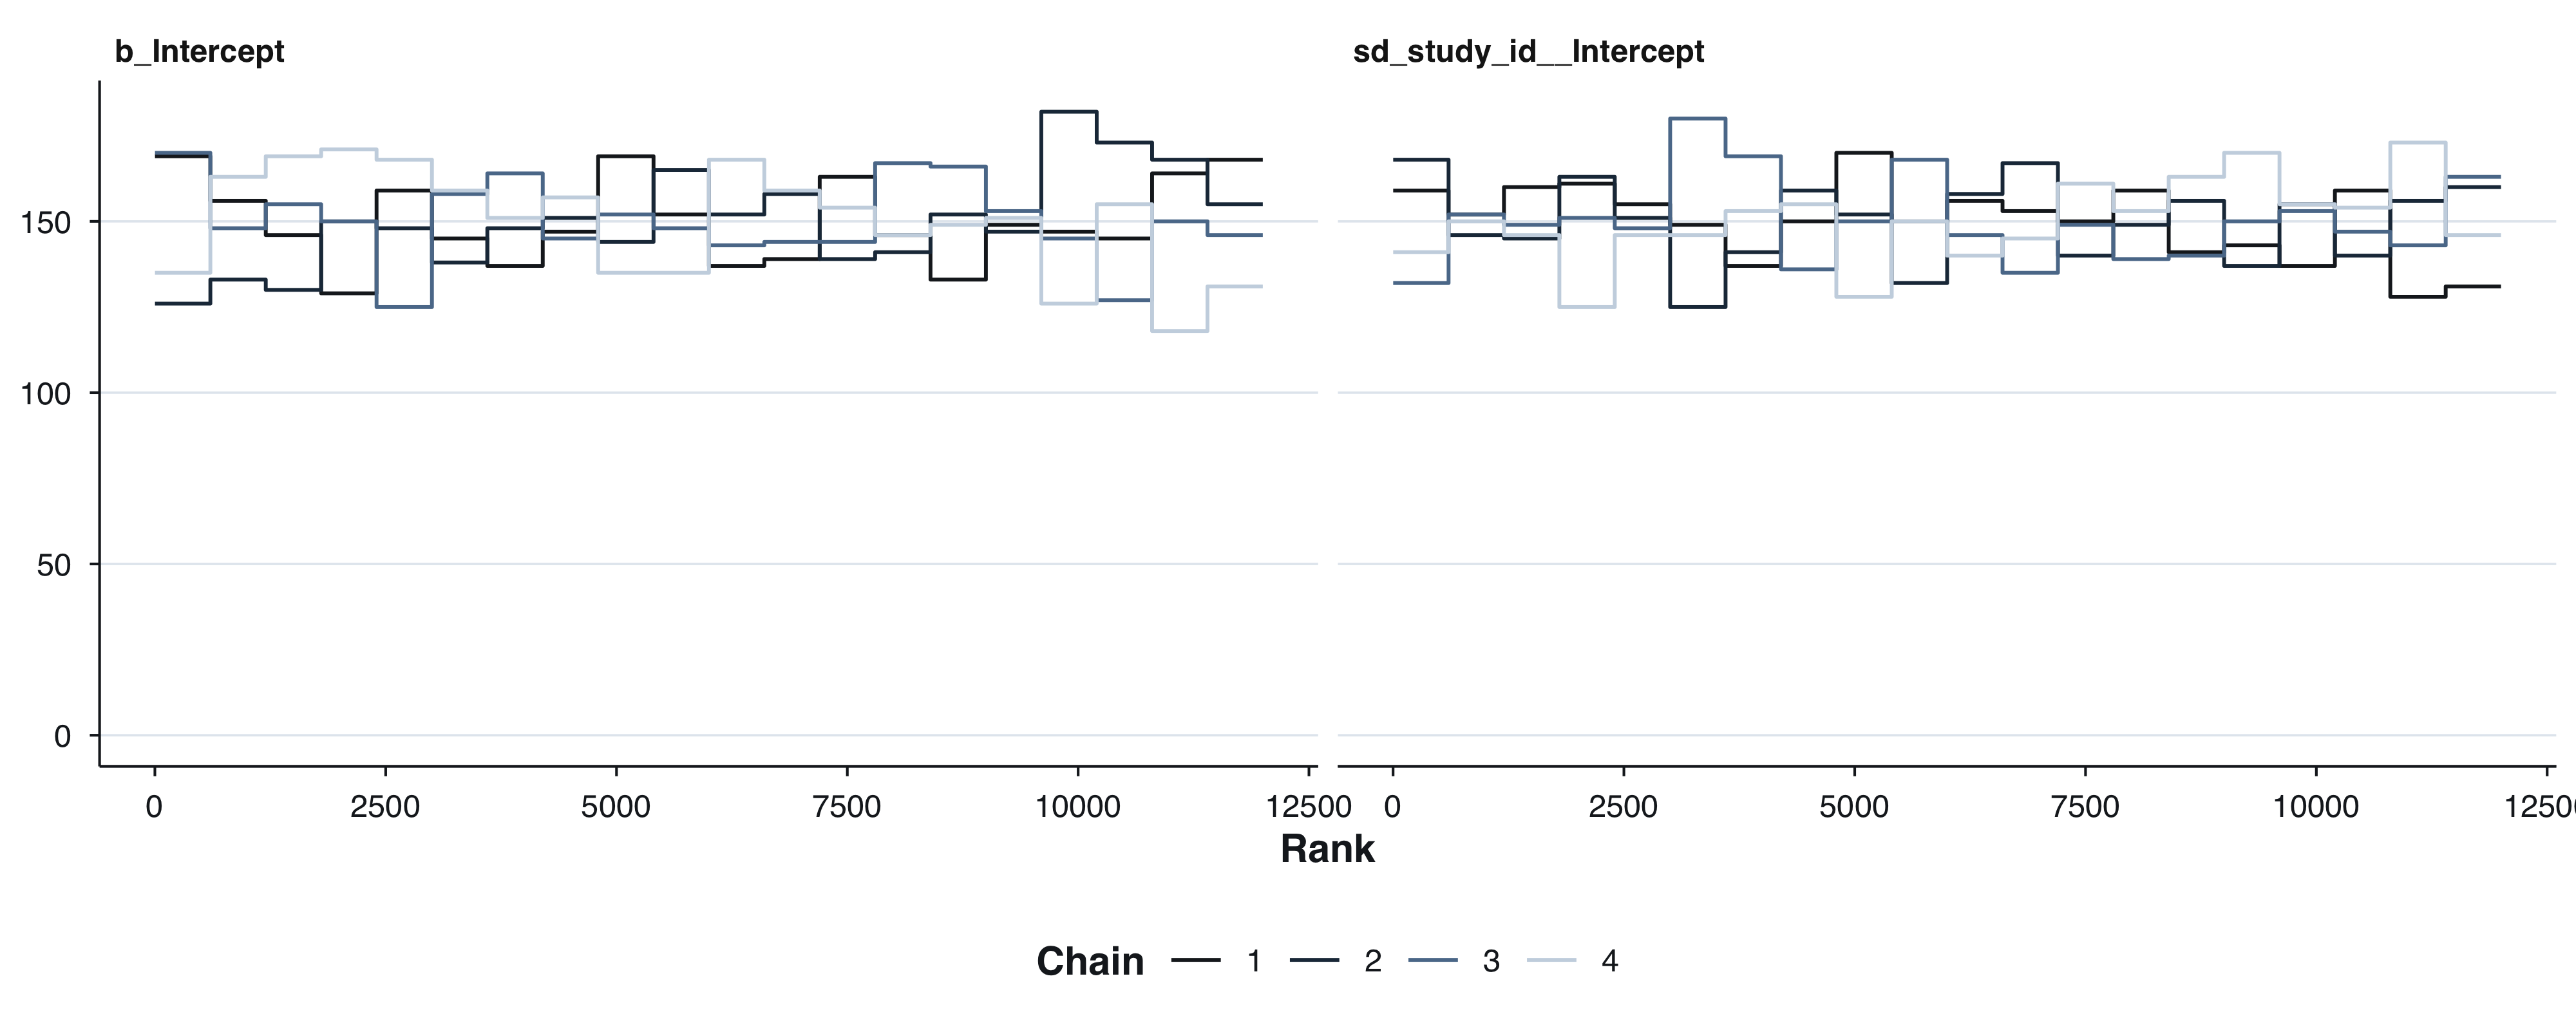
\includegraphics[keepaspectratio]{index_files/figure-latex/notebooks-mortality-analysis-fig-rank-sens-output-1.png}}

}

\caption{\label{fig-rank-sens}Rank histograms for key parameters of the
sensitivity (n=140) model.}

\end{figure}%

\textsubscript{Source:
\href{https://lewis-id-lab.github.io/ttp-bacteremia-meta-analysis/notebooks/mortality-analysis-preview.html\#cell-fig-rank-sens}{Time-to-Positivity
and Mortality in Bacteremia}}

\begin{figure}[H]

\centering{

\pandocbounded{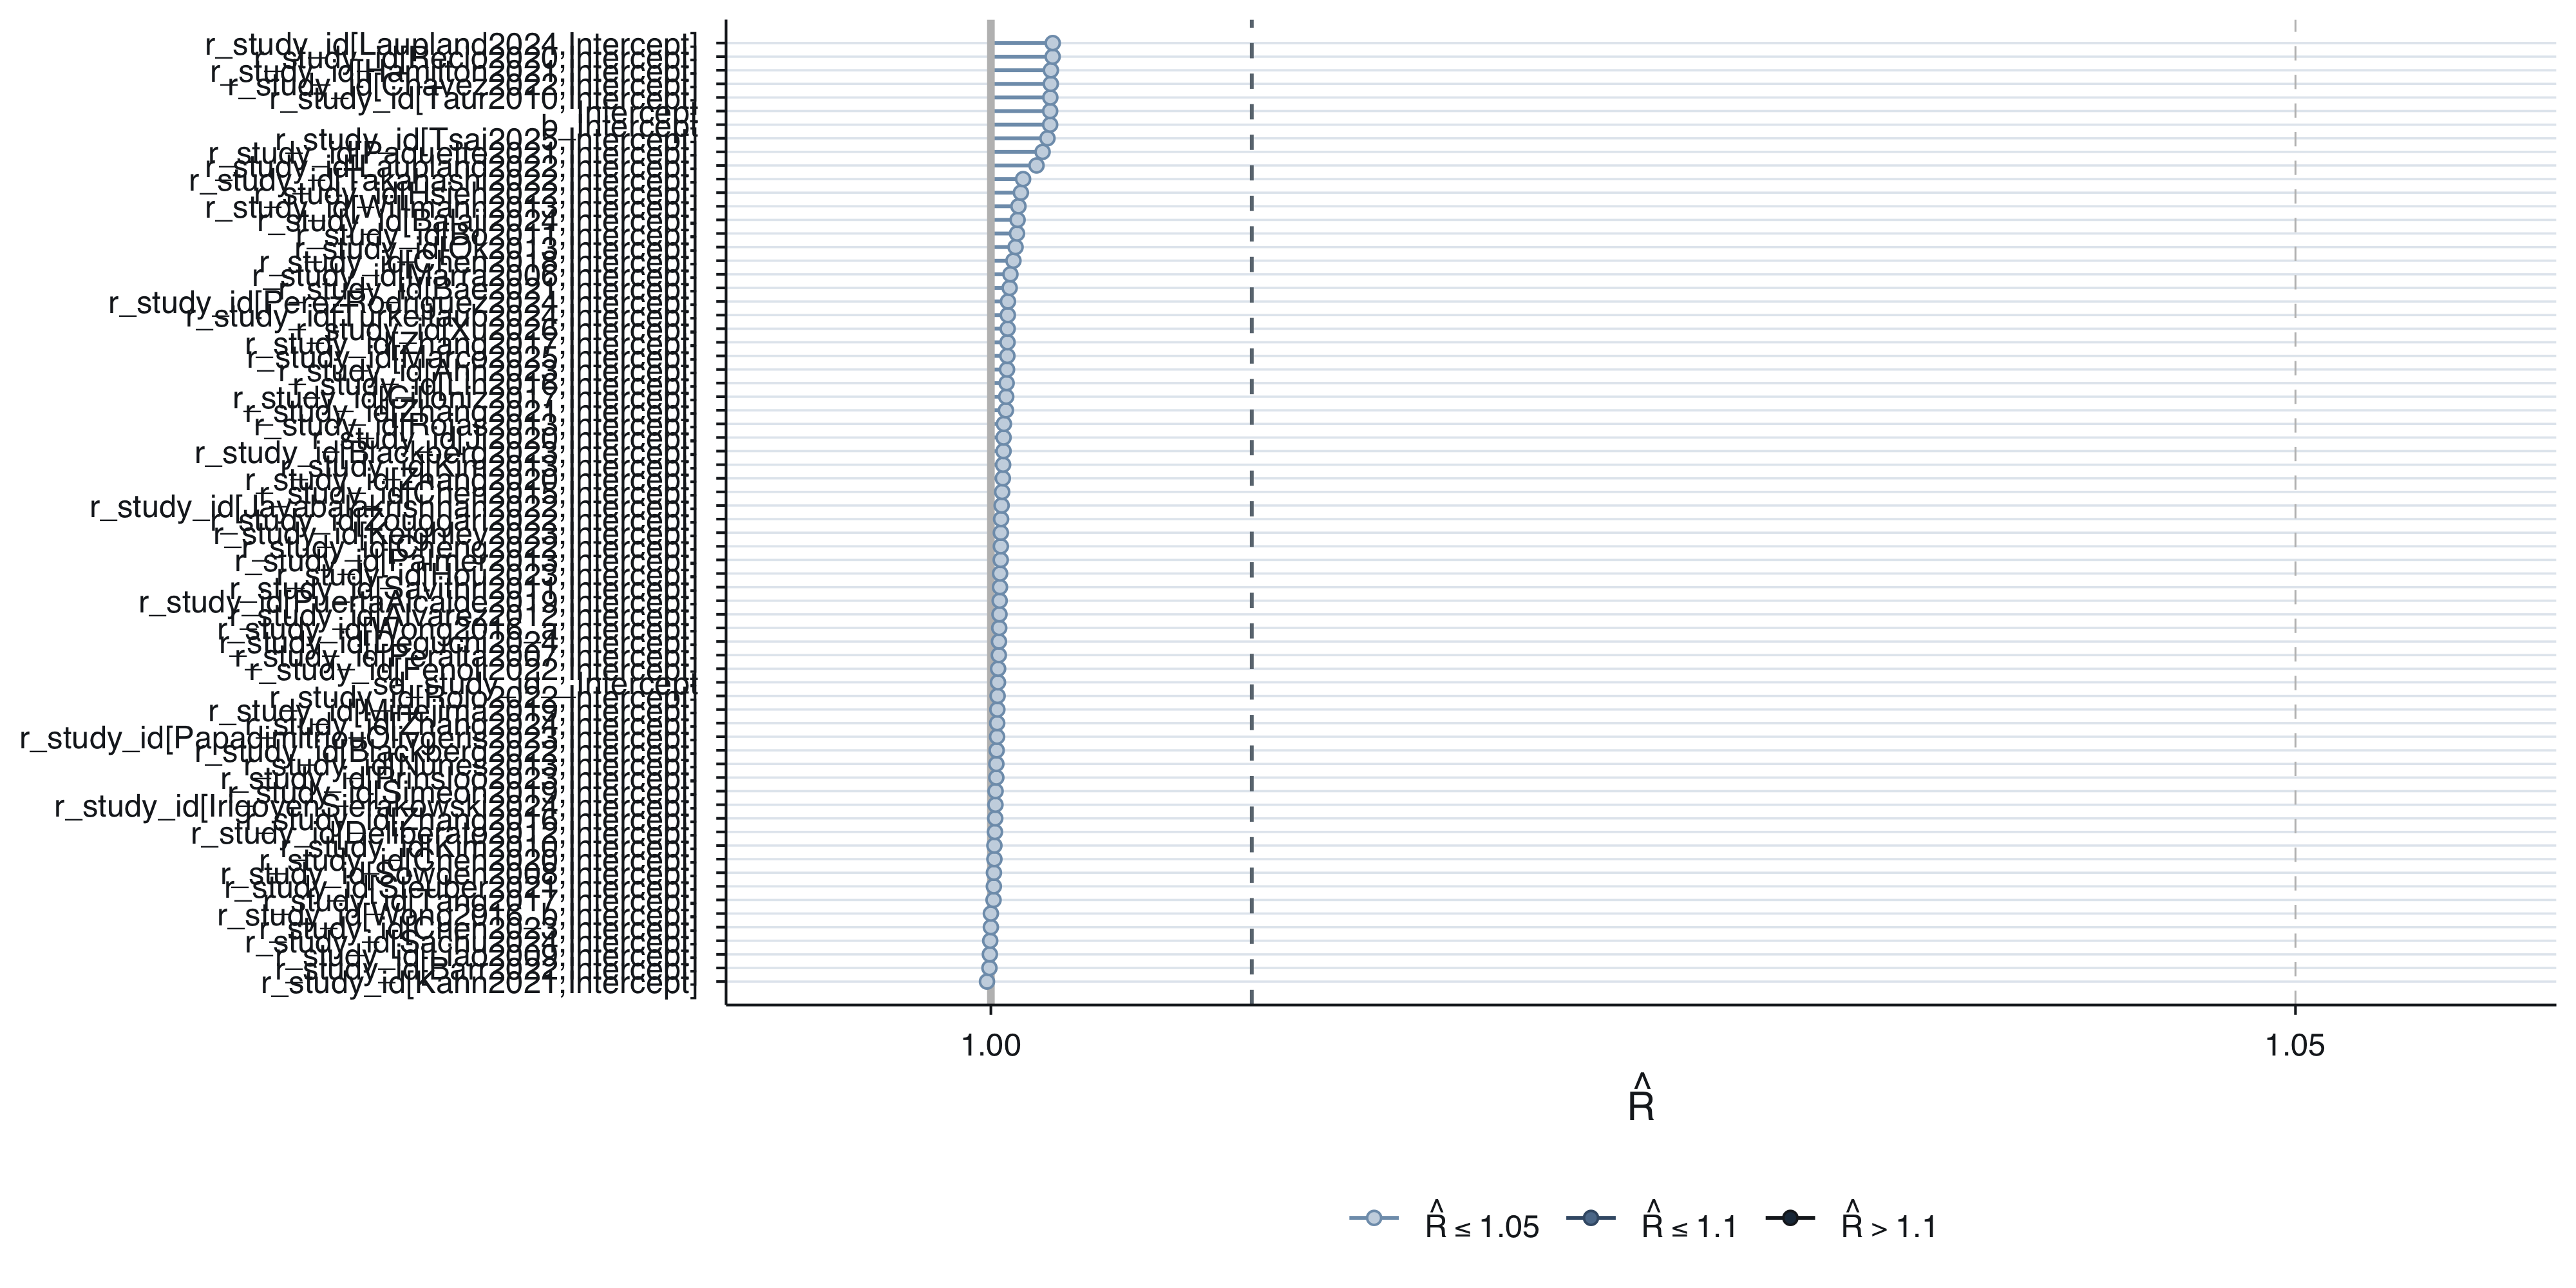
\includegraphics[keepaspectratio]{index_files/figure-latex/notebooks-mortality-analysis-fig-rhat-sens-output-2.png}}

}

\caption{\label{fig-rhat-sens}R̂ dot plot for all parameters of the
sensitivity (n=140) model. All values should fall below 1.01 (dashed
line).}

\end{figure}%

\textsubscript{Source:
\href{https://lewis-id-lab.github.io/ttp-bacteremia-meta-analysis/notebooks/mortality-analysis-preview.html\#cell-fig-rhat-sens}{Time-to-Positivity
and Mortality in Bacteremia}}

\subsection*{Moderator and sensitivity
analyses}\label{moderator-and-sensitivity-analyses}
\addcontentsline{toc}{subsection}{Moderator and sensitivity analyses}

{

\begin{longtable}[]{@{}llll@{}}

\caption{\label{tbl-mods}All moderator and sensitivity analyses (primary
pool). Δ log-OR is the change in pooled log-OR per unit of the
moderator; negative values shrink the short-TTP harm signal.}

\tabularnewline

\toprule\noalign{}
Moderator & Δ log-OR & 95\% CrI & P(direction) \\
\midrule\noalign{}
\endhead
\bottomrule\noalign{}
\endlastfoot
TTP cutpoint (per 10 h) & -0.355 & {[}-0.561, -0.153{]} & 99.9\% \\
Pathogen: Gram+ vs Gram− & -0.500 & {[}-1.016, 0.024{]} & 97.0\% \\
Adjustment: adjusted vs unadjusted & 0.123 & {[}-0.385, 0.624{]} &
68.7\% \\
Publication year (per 5 yr) & -0.203 & {[}-0.414, 0.001{]} & 97.5\% \\

\end{longtable}

}

\textsubscript{Source:
\href{https://lewis-id-lab.github.io/ttp-bacteremia-meta-analysis/notebooks/mortality-analysis-preview.html\#cell-tbl-mods}{Time-to-Positivity
and Mortality in Bacteremia}}




\end{document}
